\documentclass[a4paper, 12pt]{article}
\usepackage{amsmath}
\usepackage{amsthm}
\usepackage{amsfonts}
\usepackage{amssymb}
\usepackage[italian]{babel}
\usepackage[utf8x]{inputenc}
\usepackage{mathtools}
\usepackage{listings}
\usepackage{amsfonts, mathtools, placeins, floatflt, xfrac, multirow, indentfirst, fancyhdr,
            amssymb, latexsym, amsthm, eucal, float, tabularx, mdframed, bigdelim, blkarray,
            relsize, lettrine, xcolor, tikz, caption, geometry, perpage}
\usepackage[tiny]{titlesec}
\usepackage{lmodern}
\usepackage{tikz}
\usepackage{subcaption}
\usepackage[object=vectorian]{pgfornament}
\usepackage{hyperref}
\usetikzlibrary{calc}

\newcommand{\sectionline}[2]{%
  \nointerlineskip \vspace{.5\baselineskip}\hspace{\fill}
  {\color{#1}
    \resizebox{0.5\linewidth}{2ex}
    {{%
    {\begin{tikzpicture}
    \node  (C) at (0,0) {};
    \node (D) at (9,0) {};
    \path (C) to [ornament=#2] (D);
    \end{tikzpicture}}}}}%
    \hspace{\fill}
    \par\nointerlineskip \vspace{.5\baselineskip}
  }



 \makeatletter

\def\vhrulefill#1{\leavevmode\leaders\hrule\@height#1\hfill \kern\z@}

\makeatother

\newcommand{\persendchap}{

	\center 	{\vhrulefill{0.9pt} \pgfornament[scale = 0.50, symmetry=v, ydelta = -0.5pt]{11} FINE CAPITOLO \pgfornament[scale = 0.50, ydelta=-0.5pt]{11} \vhrulefill{0.9pt} }
	\flushleft

}

%\renewcommand\thechapter{\arabic{chapter}}
\definecolor{mygreen}{RGB}{28,172,0} 
\definecolor{mylilas}{RGB}{170,55,241}

\lstloadlanguages{Matlab, Fortran}
 \lstset{
         basicstyle=\footnotesize\ttfamily, 
         numbers=left,              
         morekeywords={matlab2tikz},
         numberstyle=\tiny,        
         numbersep=5pt,           
         tabsize=2,                 
         extendedchars=true,        
         breaklines=true,           
         keywordstyle=\color{blue},
            frame=b,
         showspaces=false,          
         showtabs=false,            
         xleftmargin=17pt,
         framexleftmargin=17pt,
         framexrightmargin=5pt,
         framexbottommargin=4pt,
         showstringspaces=false     
              morekeywords=[2]{1}, keywordstyle=[2]{\color{black}},
    identifierstyle=\color{black},%
    stringstyle=\color{mylilas},
    commentstyle=\color{mygreen},%
    showstringspaces=false,
 }


\usepackage{caption}
\DeclareCaptionFont{white}{\color{white}}
\DeclareCaptionFormat{listing}{\colorbox[cmyk]{0.43, 0.35, 0.35,0.01}{\parbox{\textwidth}{\hspace{15pt}#1#2#3}}}
\captionsetup[lstlisting]{format=listing,labelfont=white,textfont=white, singlelinecheck=false, margin=0pt, font={bf,footnotesize}}
\newtheorem{mydef}{Definizione}
\begin{document}
\renewcommand{\lstlistingname}{Codice}

\begin{titlepage}
	\begin{center}
 		
\includegraphics[scale=0.30]{logo/LOGO}\\
				
		\vspace{1.0cm}
		\Huge  Relazione \\ \vspace{0.3cm} di\\ \vspace{0.3cm} Metodi Numerici per la Grafica \\
		\vspace{1.5 cm}
		\Large  Di \vspace{0.2cm} \\ Federico Schipani 

		 \vfill                   
      A.A. 2017-2018
      \vspace{1cm}

      \begin{tikzpicture}
    \node  (C) at (0,0) {};
    \node (D) at (9,0) {};
    \path (C) to [ornament=70] (D);
    \end{tikzpicture}
      \vfill   
	\end{center}
\end{titlepage}

\tableofcontents

\listoffigures
 
\lstlistoflistings

\newpage
%\vspace{30mm}

%\begin{tikzpicture}[every node/.style={inner sep=0pt}]
%\node[text width=8cm,align=center](Text){%
%
%
%La matematica è una delle manifestazioni più significative dell'amore per la sapienza. Come tale è caratterizzata da un lato da una grande libertà, 
%dall'altro dall'intuizione che il mondo è fatto di cose visibili e invisibili e la matematica ha forse una capacità, unica fra le altre scienze, 
%di passare dall'osservazione delle cose visibili all'immaginazione delle cose invisibili. Questo forse è il segreto della forza della matematica.
%
%
%\bigskip
%
%\vspace{24pt}
%  Ennio De Giorgi
%} ;
%\node[shift={(-1cm,1cm)},anchor=north west](CNW)  at (Text.north west)
%               {\pgfornament[width=2cm]{61}};
%\node[shift={(1cm,1cm)},anchor=north east](CNE)   at (Text.north east)
%               {\pgfornament[width=2cm,symmetry=v]{61}};
%\node[shift={(-1cm,-1cm)},anchor=south west](CSW) at (Text.south west)
%               {\pgfornament[width=2cm,symmetry=h]{61}};
%\node[shift={(1cm,-1cm)},anchor=south east](CSE)  at (Text.south east)
%               {\pgfornament[width=2cm,symmetry=c]{61}};
%\pgfornamenthline{CNW}{CNE}{north}{87}
%\pgfornamenthline{CSW}{CSE}{south}{87}
%\pgfornamentvline{CNW}{CSW}{west}{87}
%\pgfornamentvline{CNE}{CSE}{east}{87}
%\end{tikzpicture}
%
%
%\titleformat{\chapter}[display]
%  {\normalfont\huge\bfseries\raggedleft}
%  {\begin{tikzpicture}
%  \node[text width=3cm,align=center] (chapnum)
%    {\fontsize{100}{130}\color{gray}\selectfont\thechapter};%
%  \node[shift={(-1cm,1cm)},anchor=north west](CNW)
%    at (chapnum.north west) {\pgfornament[width=1.75cm]{61}};
%  \node[shift={(1cm,1cm)},anchor=north east](CNE)
%    at (chapnum.north east) {\pgfornament[width=1.75cm,symmetry=v]{61}};
%  \node[shift={(-1cm,-1cm)},anchor=south west](CSW)
%    at (chapnum.south west) {\pgfornament[width=1.75cm,symmetry=h]{61}};
%  \node[shift={(1cm,-1cm)},anchor=south east](CSE)
%    at (chapnum.south east) {\pgfornament[width=1.75cm,symmetry=c]{61}};
%  \end{tikzpicture}
%  }
%  {20pt}
%  {\Huge}

\section{La Base delle B-Spline}

Dato un vettore esteso dei nodi
$$ \mathbf{t} =  \left\{ \underbrace{t_{0}, \dots, t_{k-2}}_{k-1}, \underbrace{t_{k-1}, \dots, t_{n+1}}_{\tau_0, \tau_1, \dots, \tau_L}, \underbrace{t_{n+2}, \dots, t_{n+k}}_{k-1} \right\} $$
con
$$\mathbf{t_0} \leq t_1 \leq \dots t_{k+1} < t_k \dots < t_{n+1} \leq t_{n+2} \leq \dots \leq t_{n+k}$$
possiamo definire la base delle \textit{B-Spline} su nodi semplici tramite la relazione ricorrente di \textit{Cox - De Boor}.
\begin{mydef}
  Le \textit{B-Spline} di ordine $1$, oppure grado $0$ sono definite come:
$$N_{i, 1}(t) = \begin{cases} 1, & \text{se } t\in[t_i, t_{i+1}] i = 0, \dots, n+k-1 \\ 0, & \text{altrimenti} \end{cases}$$
  Altrimenti le \textit{B-Spline} di ordine $r \leq k$ sono definite ricorsivamente, per $r > 1$, come:
  $$N_{i, r}(t) = \omega_{i,r}(t)N_{i, r-1}(t) + [1-\omega_{i+1, r}(t)]N_{i+1, r-1}$$
  dove
$$\omega_{i,r}(t) = \begin{cases} \frac{t-t_i}{t_{i+r-1}-t_i}, & \text{se } t<t_{i+r-1} \\ 0, & \text{altrimenti} \end{cases}$$
\end{mydef}
Le \textit{B-Spline} possono anche essere definite su una partizione nodale la cui molteplicità $m_i$ di un generico nodo $\tau_i$ è più alta di $1$,
quindi su nodi multipli. In questo caso il vettore esteso dei nodi diventa:
$$ \mathbf{t} =  \left\{ \underbrace{t_{0}, \dots, t_{k-2}}_{k-1}, \underbrace{t_{k-1}, \dots, t_{n+1}}_{\tau_0, \tau_1, \dots, \tau_1 \dots, \tau_L}, \underbrace{t_{n+2}, \dots, t_{n+k}}_{k-1} \right\} $$
con $\tau_i$ ripetuto a seconda della sua molteplicità $m_i$ con $i = 1, \dots, L-1$ in $\mathbf{t}$, e
$$\mathbf{t_0} \leq t_1 \leq \dots t_{k+1} \leq  t_k \dots \leq  t_{n+1} \leq t_{n+2} \leq \dots \leq t_{n+k}$$
La definizione della base delle \textit{B-Spline} di \textit{Cox - De Boor} non cambia, ma bisogna stare attenti in quanto 
$\omega_{i,r}(t)$ può diventare nullo per qualche valore $r$  a causa dei nodi multipli.
In Codice \ref{code:functioncoxdeboor} sono mostrate le due funzioni che calcolano le basi di \textit{Cox - De Boor}, realizzate senza l'utilizzo delle funzioni del 
\textit{Curve Fitting Toolbox}.
\lstinputlisting[label=code:functioncoxdeboor, firstline=17, language=Matlab, caption = Calcolo delle basi di Cox De Boor]{code/cox_de_boor_basis.m}
La funzione \texttt{calc\_omega} di Codice~\ref{code:functioncoxdeboor} si può spiegare in questo modo. Dati in input
l'indice $i$, l'ordine $r$, il punto in cui si vuole calcolare la spline $t\_star$ ed il vettore esteso dei nodi $\mathbf{t}$ si occupa di calcolare i valori $\omega_{i, r}(t)$.
Il controllo iniziale \texttt{t(i) == t(i+r-1)} serve a gestire il caso di nodi multipli. In questa particolare condizione possiamo trovarci a gestire casi in cui il denominatore di $\frac{t - t_i}{t_{i+1-r}-t_i}$ è uguale a $0$; quindi
$\omega_{i,r}(t)$ dev'essere posto a $0$. 
La seconda funzione in Codice~\ref{code:functioncoxdeboor} è \texttt{de\_boor\_basis} che effettua il calcolo delle basi delle B-Spline. 
La condizione booleana a riga 16, 17 e 18 serve a verificare che, nel caso 
in cui l'ordine della spline sia $1$, ci si trovi all'interno dell'intervallo $[t_i, t_{i+1} )$. Bisogna però fare attenzione al caso in cui 
il punto $t = t\_star$ di $N_{i, k}(t)$ si trovi nell'ultimo intervallo. Questo ha reso necessario introdurre un ulteriore controllo per fare in modo che venga 
preso in considerazione anche l'ultimo valore dell'ultimo intervallo.
\subsection{Esempi di basi}
L'esempio più immediato di base è quello dove il vettore esteso dei nodi è uniforme, in questo caso abbiamo preso $\mathbf{t} = [0, 1, 2, 3, 4, 5, 6, 7, 8, 9]$ e $k = 5$, otterremo quindi $5$
funzioni di base visualizzate in Figura~\ref{fig:first_basis}.
\begin{figure}[]
  \centering
  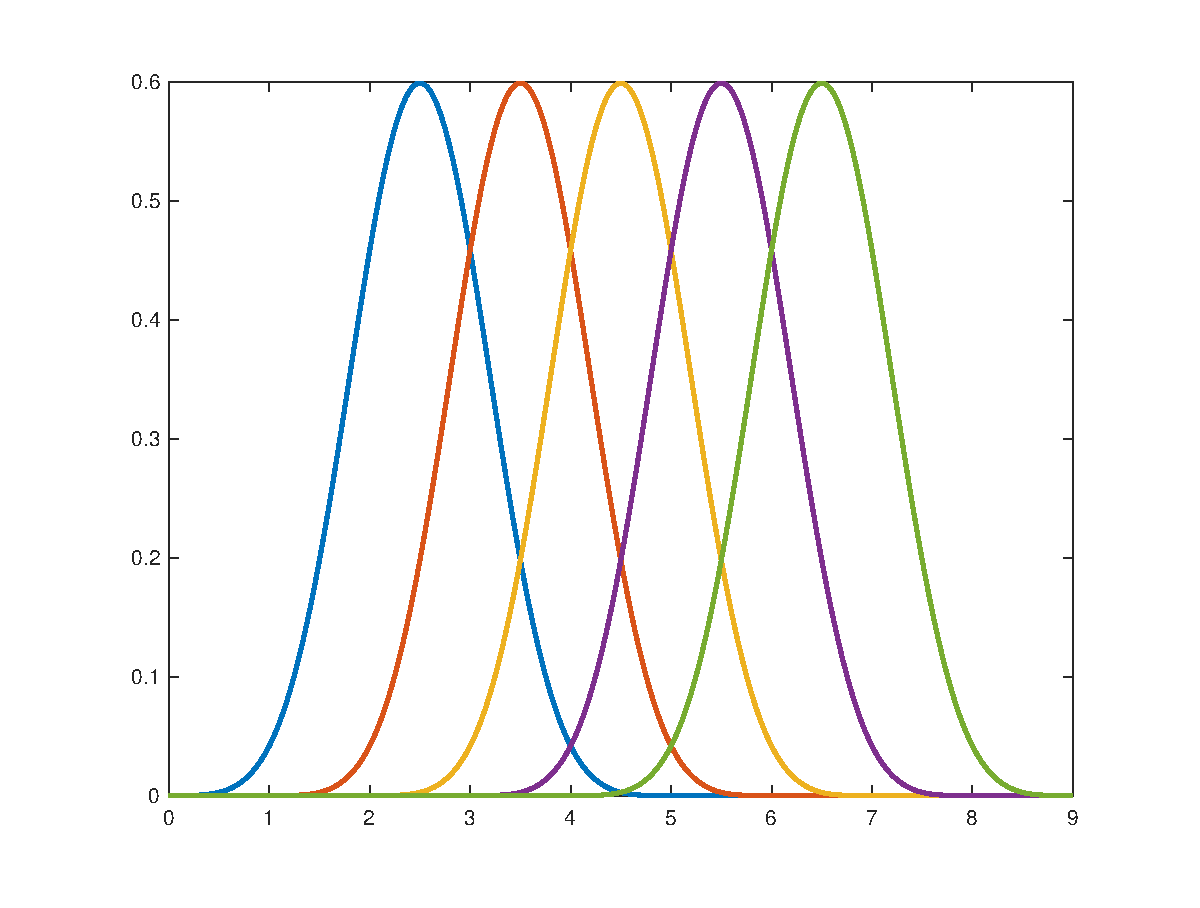
\includegraphics[width=0.75\textwidth]{figure/uniform_not_multiple_basis.eps}
  \caption{Base con $\mathbf{t} = [0, 1, 2, 3, 4, 5, 6, 7, 8, 9]$ e $k = 5$}
  \label{fig:first_basis}
\end{figure} 

Cambiando il vettore esteso dei nodi $\mathbf{t}$ otteniamo basi per le \textit{B-Spline} con regolarità diversa.
In Figura~\ref{fig:animals} viene mostrato cosa succede tenendo fissato il numero di nodi e l'ordine e aumentato la molteplicità del nodo $4$.

\begin{figure}[]
  \centering
  \begin{subfigure}[b]{0.3\textwidth}
    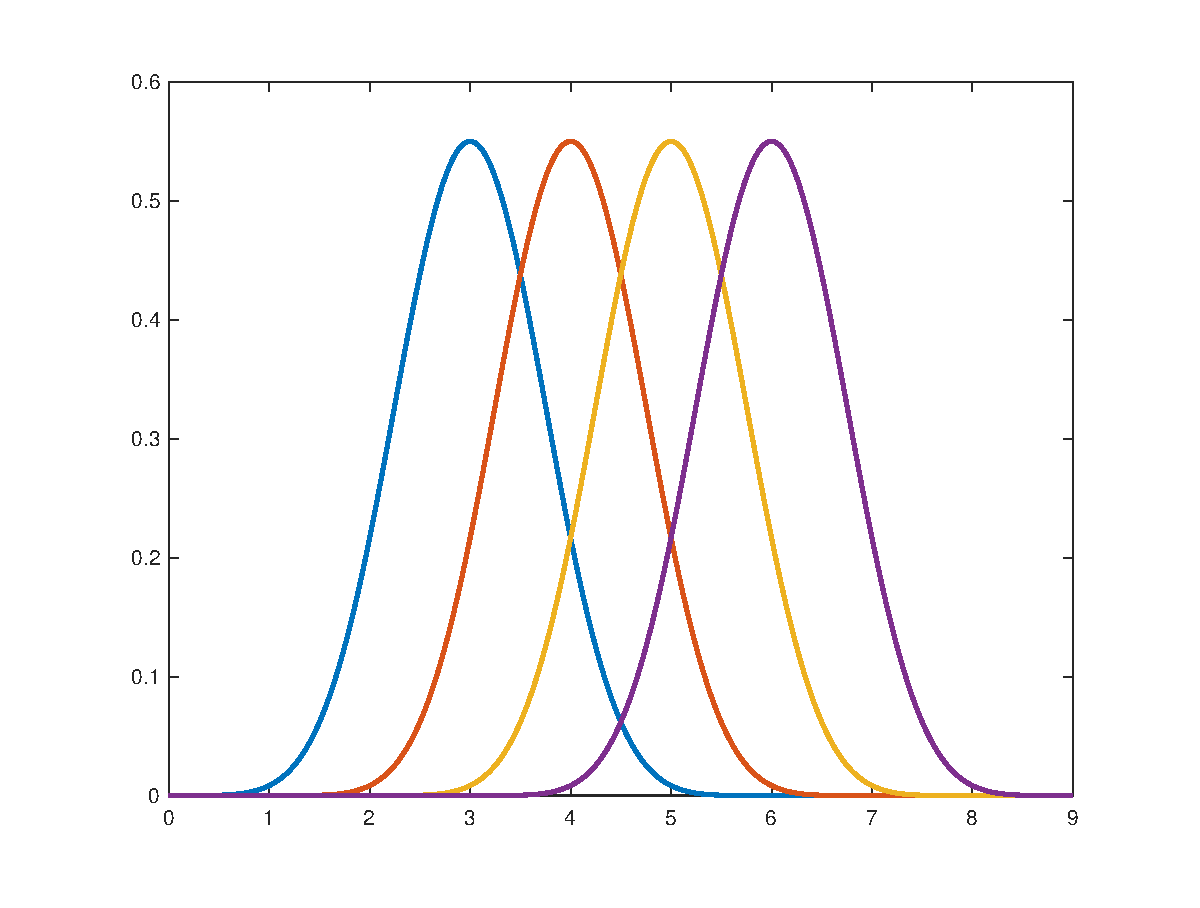
\includegraphics[width=\textwidth]{figure/6_41.eps}
    \caption{$\mathbf{t} = [0, 1, 2, 3, 4, 5, 6, 7, 8, 9]$}
    \label{fig:641}
  \end{subfigure}
  \begin{subfigure}[b]{0.3\textwidth}
      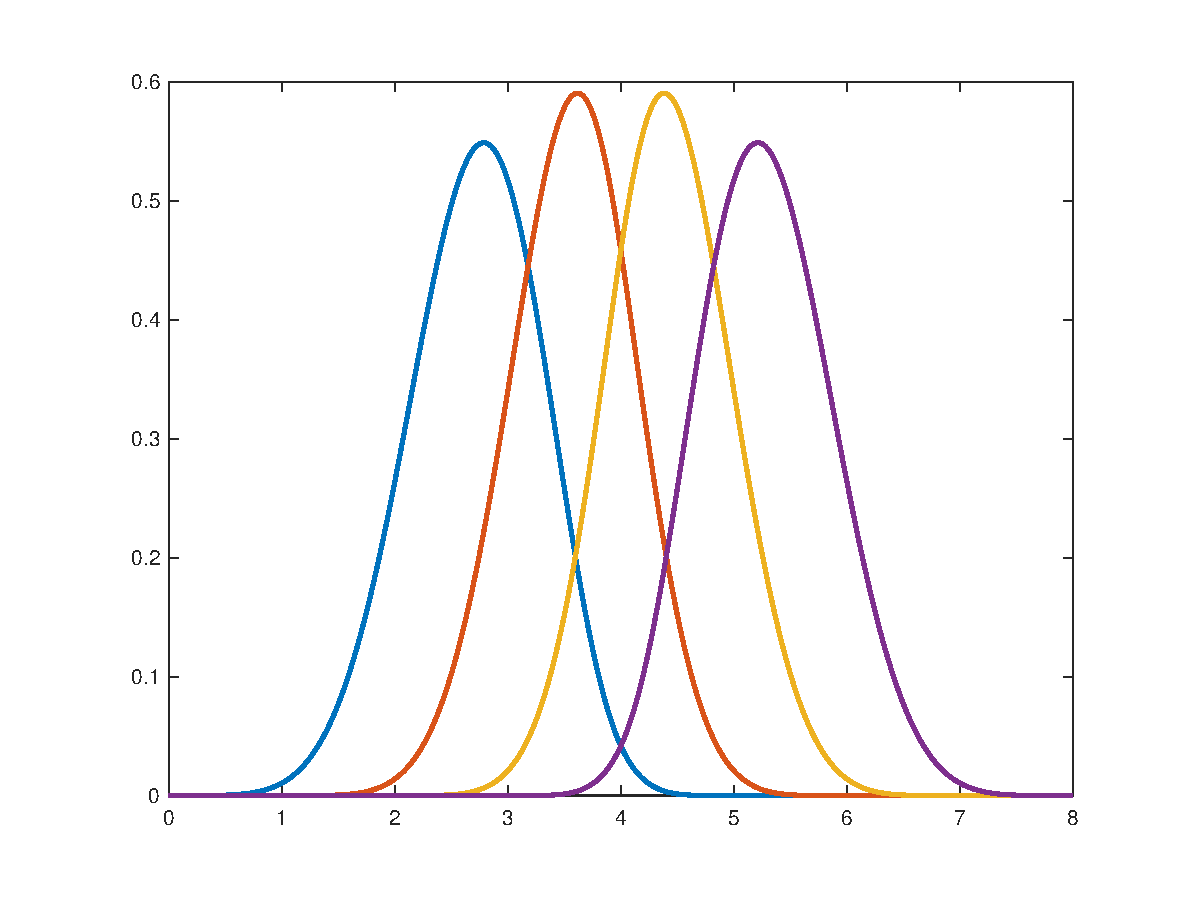
\includegraphics[width=\textwidth]{figure/6_42.eps}
      \caption{$\mathbf{t} = [0, 1, 2, 3, 4, 4, 5, 6, 7, 8]$}
      \label{fig:642}
  \end{subfigure}
  \begin{subfigure}[b]{0.3\textwidth}
      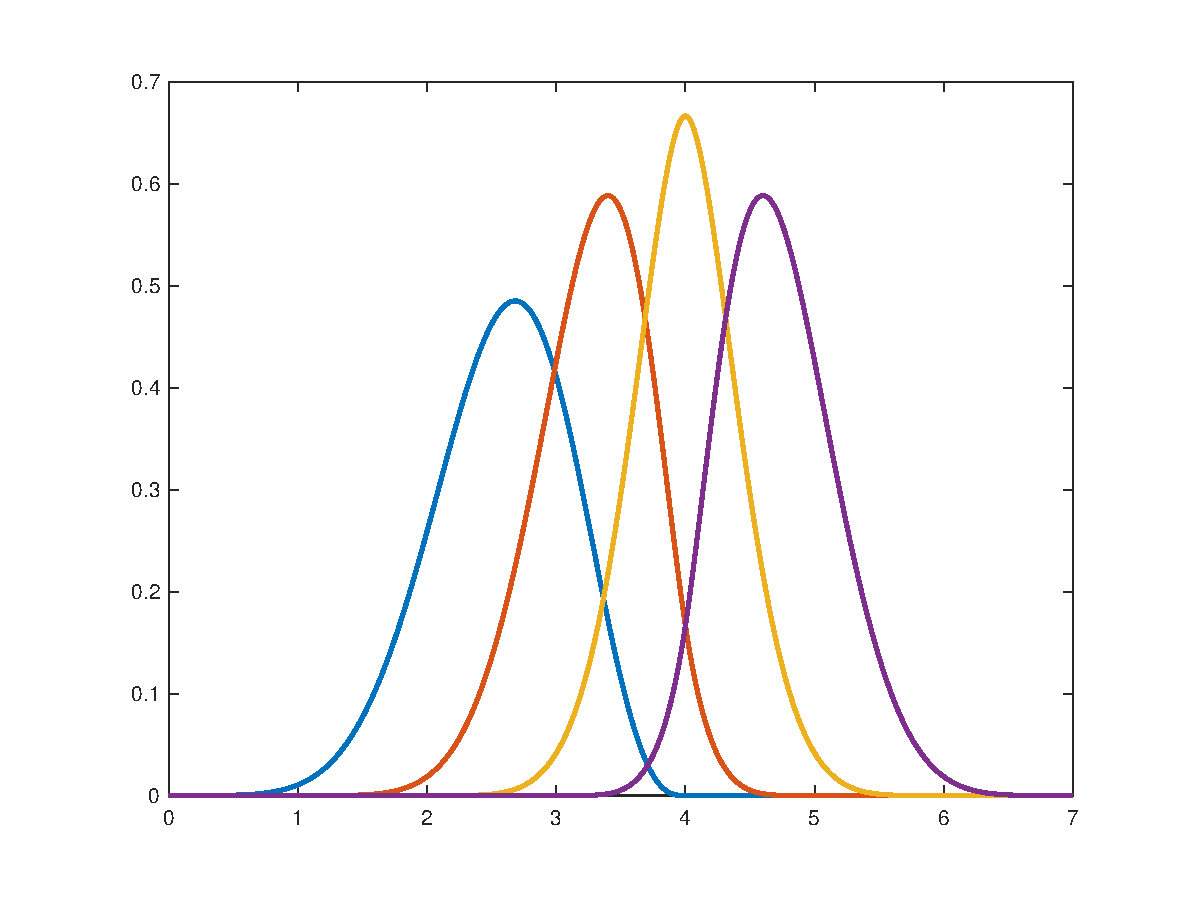
\includegraphics[width=\textwidth]{figure/6_43.eps}
      \caption{$\mathbf{t} = [0, 1, 2, 3, 4, 4, 4,5, 6, 7]$}
      \label{fig:643}
  \end{subfigure}
  \begin{subfigure}[b]{0.3\textwidth}
      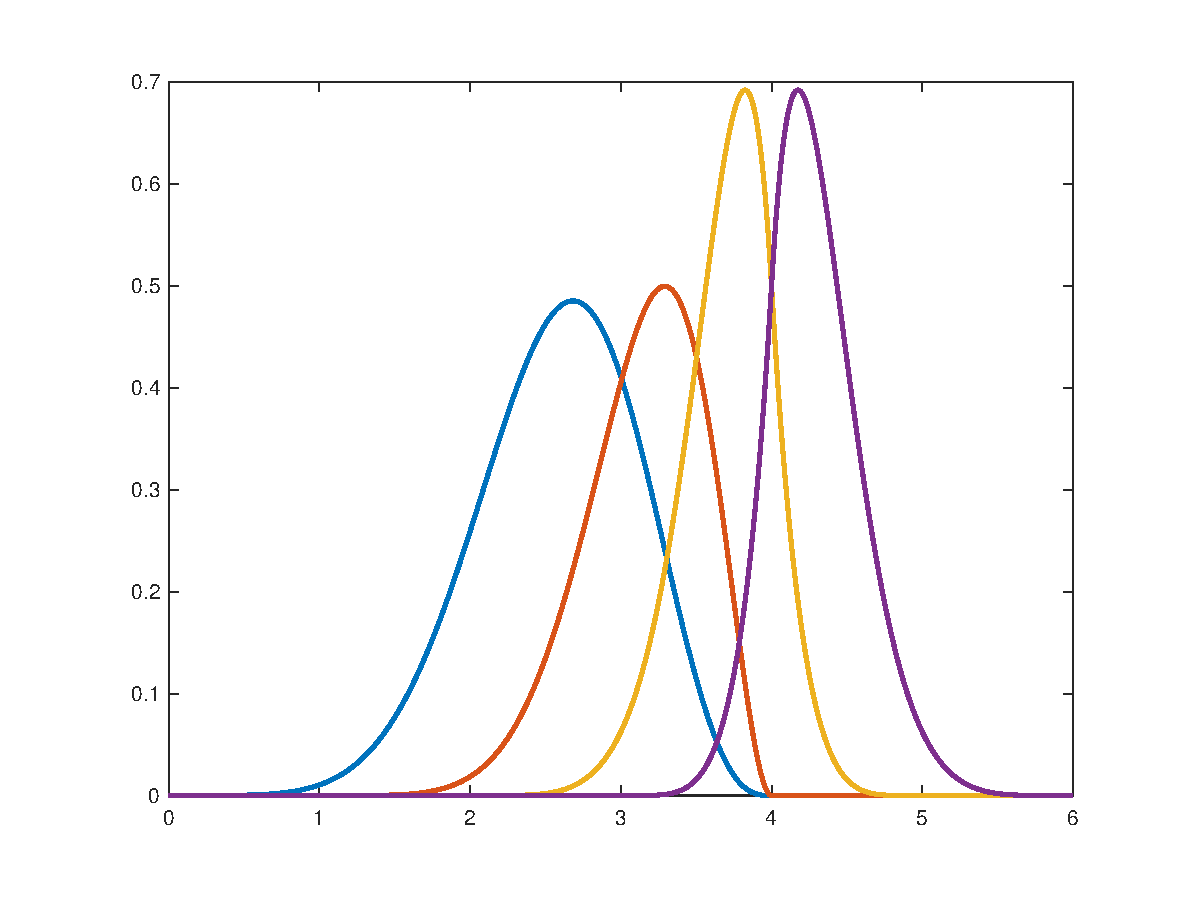
\includegraphics[width=\textwidth]{figure/6_44.eps}
      \caption{$\mathbf{t} = [0, 1, 2, 3, 4, 4, 4, 4, 5, 6]$}
      \label{fig:644}
  \end{subfigure}
  \begin{subfigure}[b]{0.3\textwidth}
    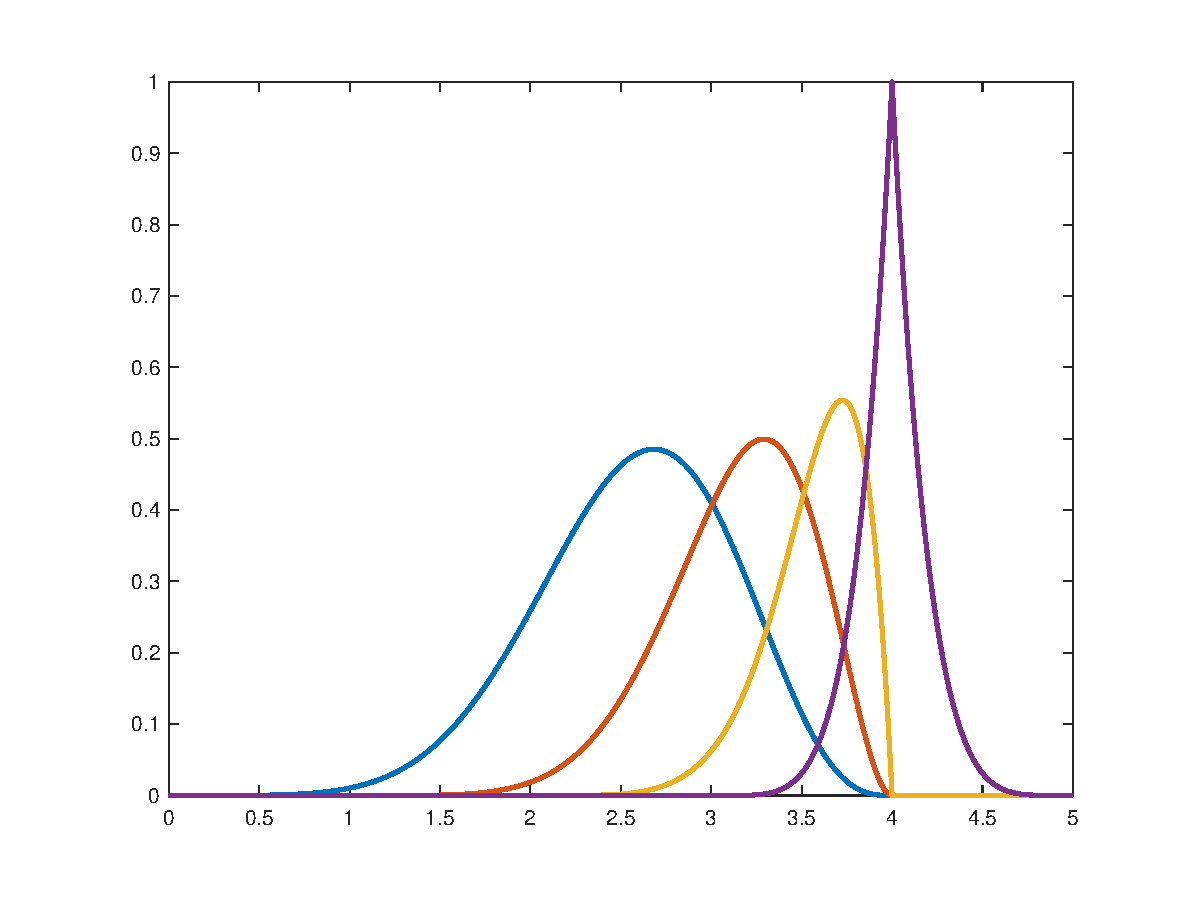
\includegraphics[width=\textwidth]{figure/6_45.eps}
    \caption{$\mathbf{t} = [0, 1, 2, 3, 4, 4, 4, 4, 5]$}
    \label{fig:645}
  \end{subfigure}
  \caption{Base con nodi multipli di ordine 6}\label{fig:animals}
\end{figure}

Un caso particolare della base delle \textit{B-Spline} sono i polinomi di \textit{Bernstein}. Questi ultimi si ottengono quando, 
dato $[a, b] = [\tau_0, \tau_L]$, la partizione nodale estesa è formata solamente da $a$ ripetuto $k$ volte
e $b$ ripetuto altrettante $k$ volte. In Figura~\ref{fig:bernstein} è mostrato un esempio di base ottenuta con 
i polinomi di \textit{Besrnstein} di grado $5$.

\begin{figure}[]
  \centering
  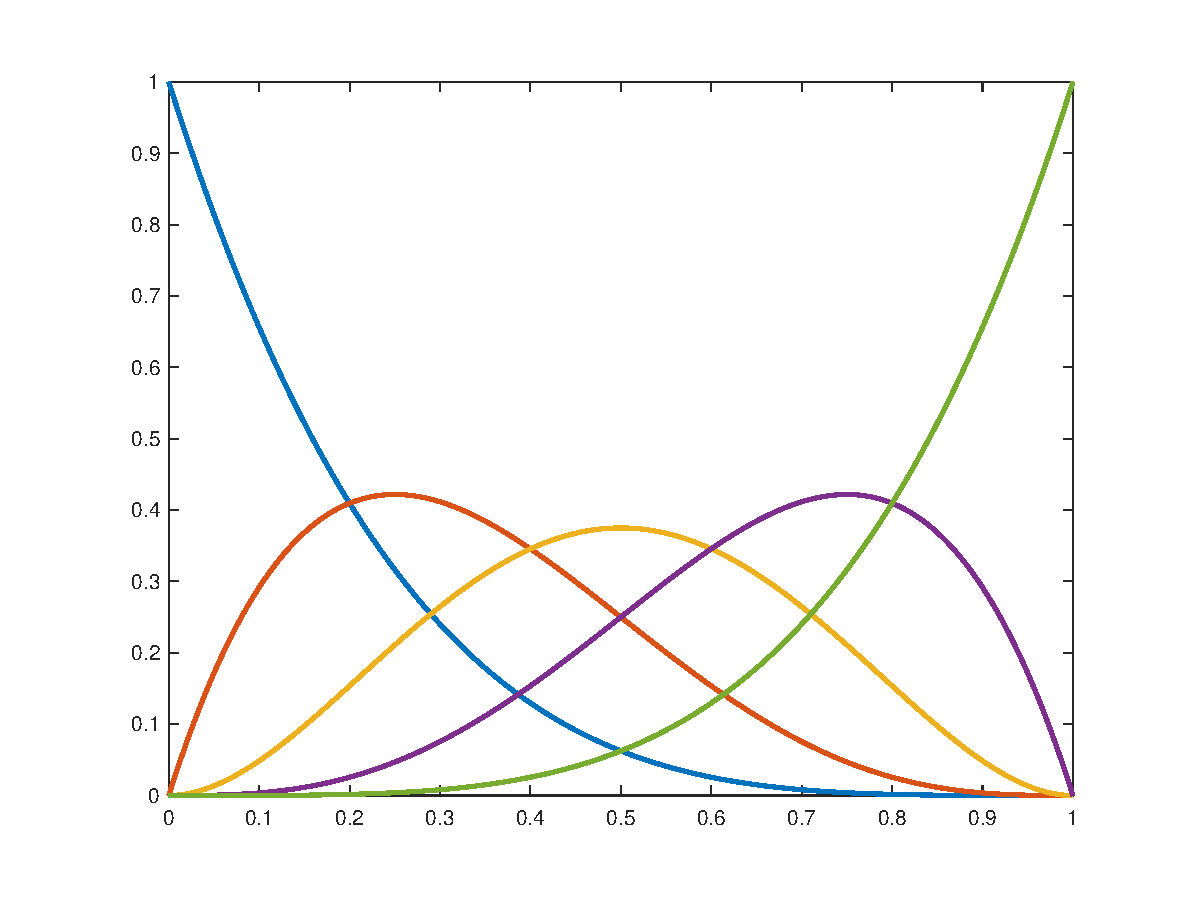
\includegraphics[width=0.75\textwidth]{figure/bernstein5_from_cox_de_boor.eps}
  \caption{Base di Bernstein di ordine $5$}
  \label{fig:bernstein}
\end{figure} 

\subsection{Proprietà della base delle B-Spline}
La base delle \textit{B-Spline} gode di diverse proprietà:
\begin{enumerate}
  \item Supporto locale: $N_{i, r}(t) = 0 \text{ se } t \notin [t_i, t_{i+r}]$
  \item Non negatività: $N_{i, r}(t) \geq 0\ \forall \ t \ \in \mathbb{R}$
  \item Partizione dell'unità: $\sum_{i = 0}^{n+k-r} = 1 \ \forall \  t \ \in [t_{r-1}, t_{n+1+k-r}] \text{ con } r = 1 \dots k$
\end{enumerate}
\paragraph{Supporto locale}
Questa proprietà ci dice che la spline $N_{i, r}(t)$ è diversa da zero solamente nell'intervallo di nodi che va 
da $t_i$ a $t_{i+r}$. Prendiamo ad esempio le \textit{B-Spline} di ordine $k = 4$ e 
con $\mathbf{t} = [0, 0, 0, 1, 1, 2, 3, 3, 3]$. Le splines saranno le seguenti:
\begin{itemize}
  \item $N_{1, 4}(t)\neq 0\ t \in [t_1 = 0, t_5 = 1]$
  \item $N_{2, 4}(t)\neq 0\ t \in [t_2 = 0, t_6 = 2]$
  \item $N_{3, 4}(t)\neq 0\ t \in [t_3 = 0, t_7 = 3]$
  \item $N_{4, 4}(t)\neq 0\ t \in [t_4 = 1, t_8 = 3]$
  \item $N_{5, 4}(t)\neq 0\ t \in [t_5 = 1, t_9 = 3]$
\end{itemize}
Facendo un plot di questa base possiamo vedere come la proprietà di supporto locale sia verificata, in particolare in Figura~\ref{fig:local_support} sono mostrate
tutte le splines della base, mentre in Figura~\ref{fig:first_property} è mostrato un dettaglio della $N_{1, 4}(t)$ per $t = [0.85, 1.15]$.
\begin{figure}[]
  \centering
  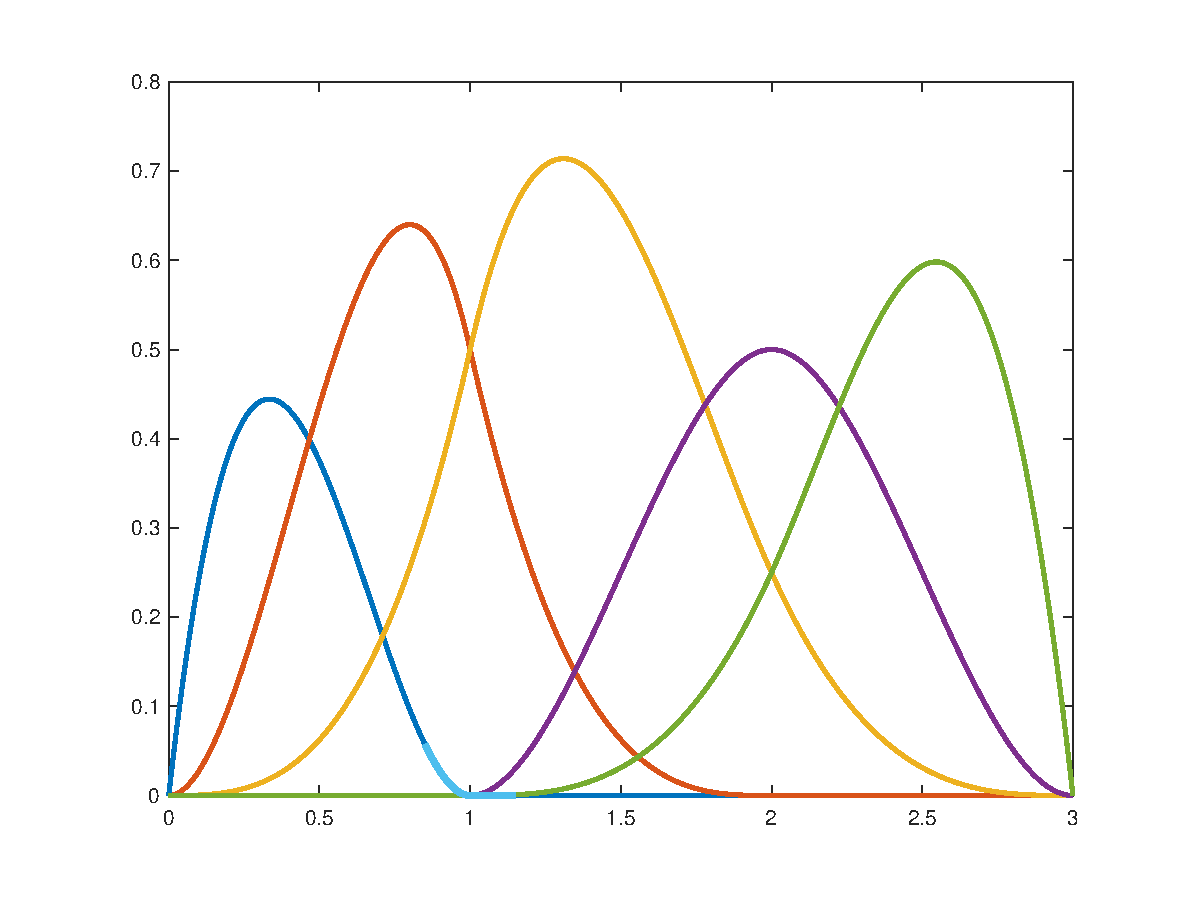
\includegraphics[width=0.75\textwidth]{figure/local_support.eps}
  \caption{Supporto locale}
  \label{fig:local_support}
\end{figure} 
\begin{figure}[]
  \centering
  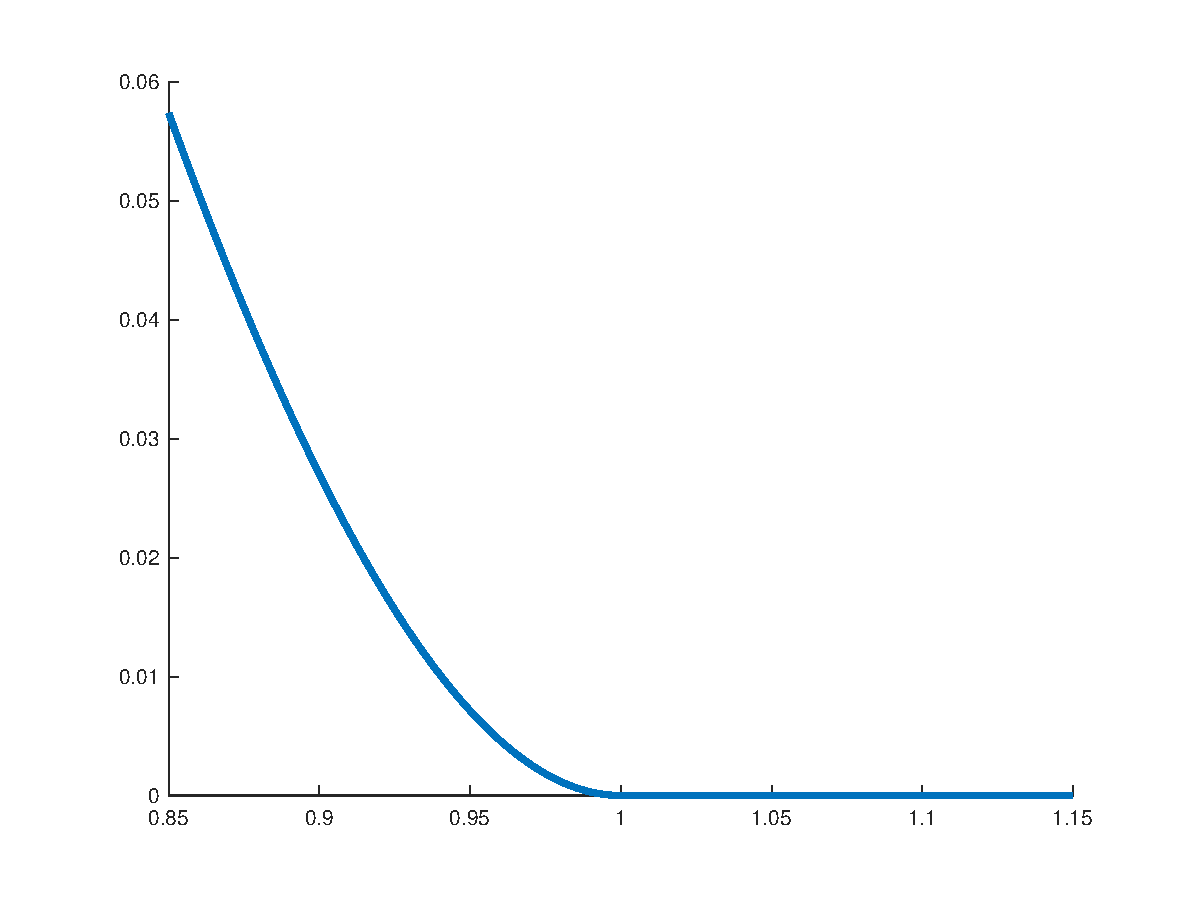
\includegraphics[width=0.75\textwidth]{figure/first_property.eps}
  \caption{Dettaglio della prima splines $N_{1, 4}(t)$ per $t = [0.85, 1.15]$}
  \label{fig:first_property}
\end{figure} 
\paragraph{Non negatività} In questo caso la proprietà è verificabile sfruttando uno qualunque dei plot mostrati in precedenza,
 ad esempio possiamo vedere che in Figura \ref{fig:local_support} nessuna delle $N_{i, r}(t)$ è negativa.
\paragraph{Partizione dell'unità} Questa proprietà ci dice che 
la somma delle funzioni di base delle \textit{B-Spline} definite sulla partizione nodale estesa $\mathbf{t}$ è uguale a 1, se si considerano nell'intervallo 
$[\tau_0, \tau_L]$.
Un esempio è mostrato in Figura~\ref{fig:unity_partition}.






\begin{figure}[]
  \centering
  \begin{subfigure}[b]{0.45\textwidth}
    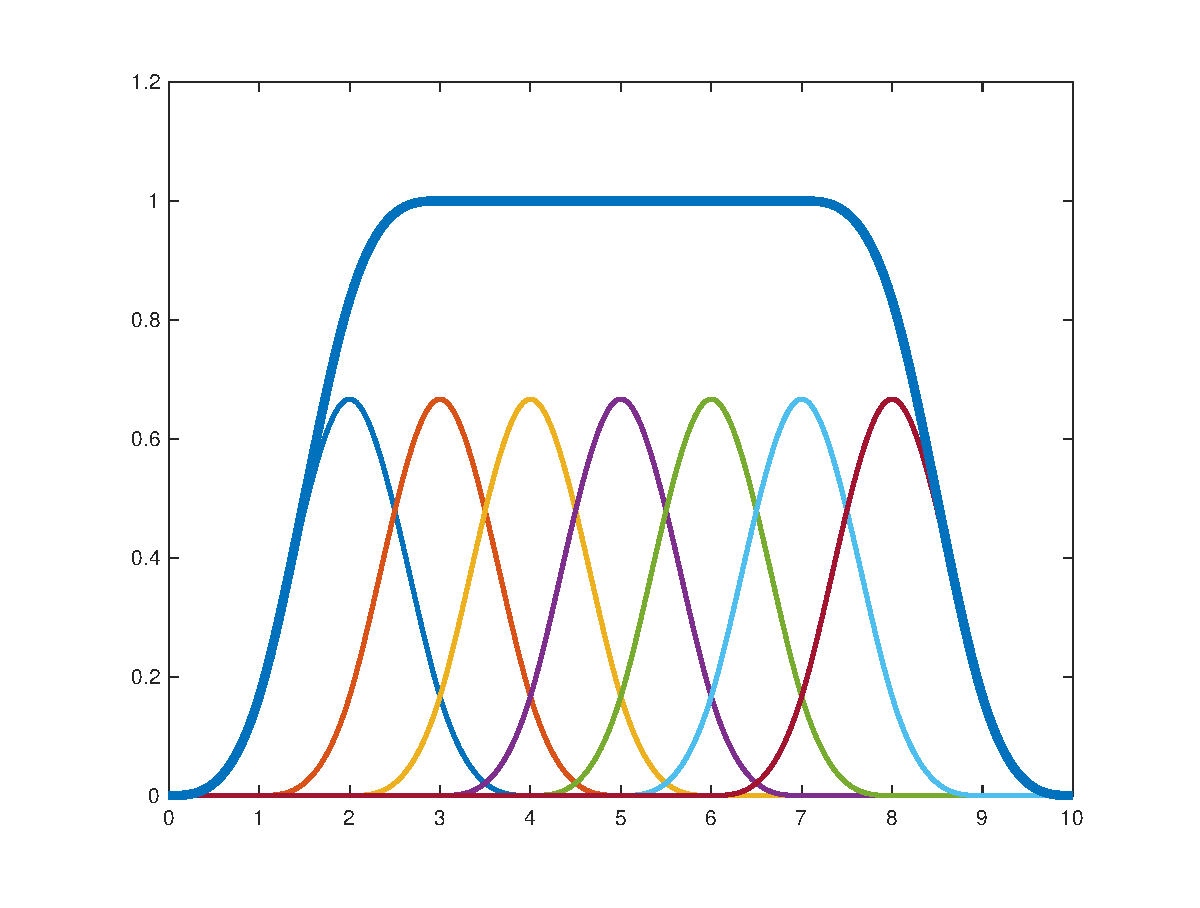
\includegraphics[width=0.75\textwidth]{figure/unity_std.eps}
    \caption{Nodi uniformi}
    \label{fig:unity_std}
  \end{subfigure}
  \begin{subfigure}[b]{0.45\textwidth}
    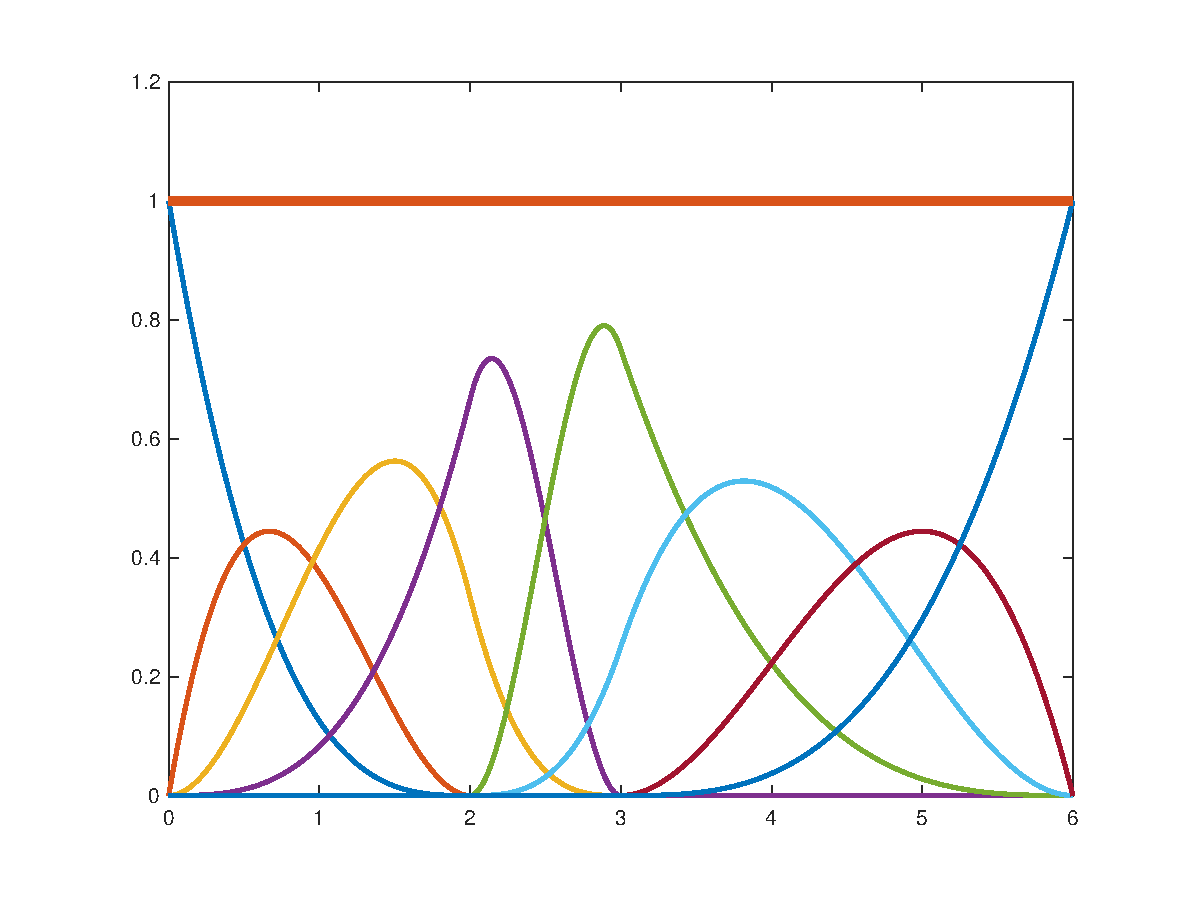
\includegraphics[width=0.75\textwidth]{figure/unity_3.eps}
    \caption{Nodi \textit{clamped}}
    \label{fig:unity_clamped}
  \end{subfigure}
  \begin{subfigure}[b]{0.5\textwidth}
    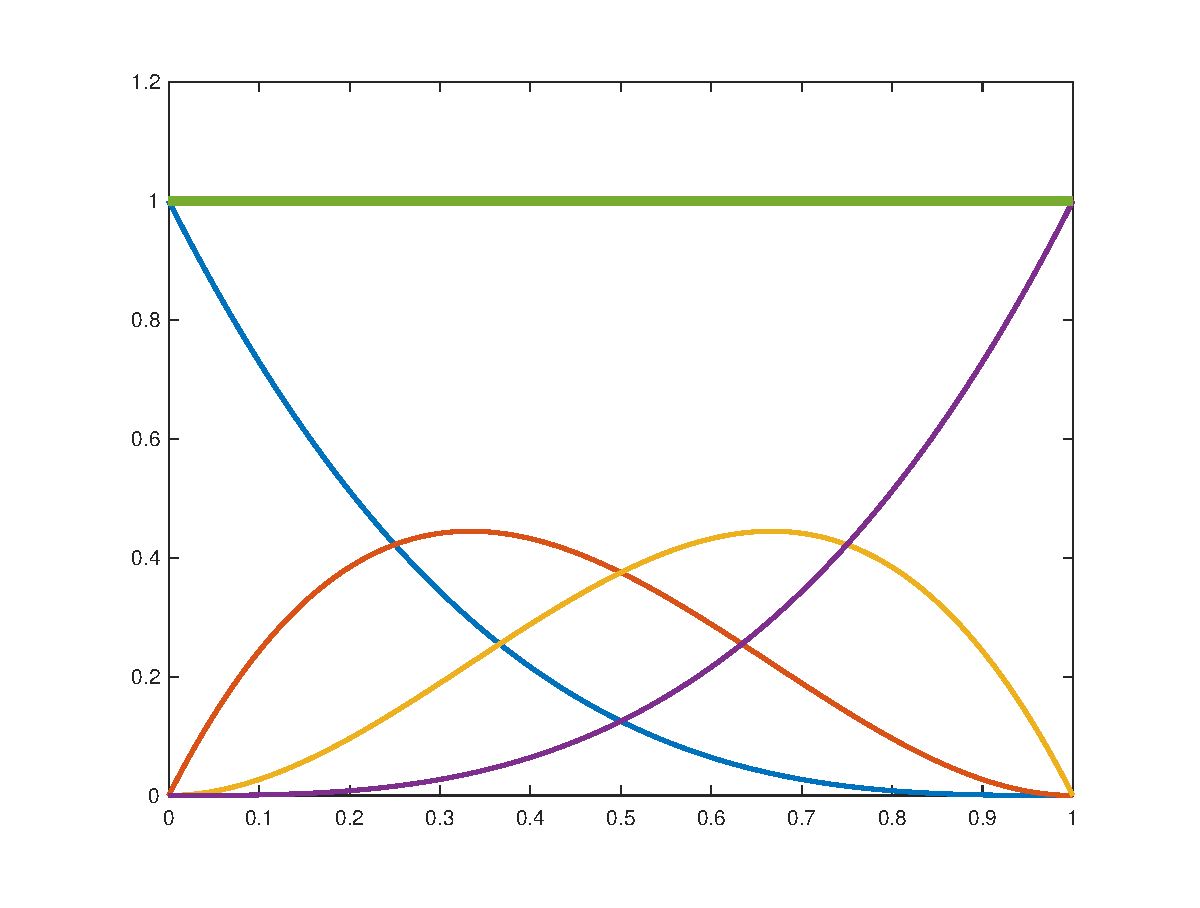
\includegraphics[width=0.75\textwidth]{figure/unity_bernstein.eps}
    \caption{Base di Bernstein}
    \label{fig:unity_bernstein}
  \end{subfigure}
  \caption{Partizione dell'unità}\label{fig:unity_partition}
\end{figure}




\section{Curve B-Spline}
A partire dalla base delle \textit{B-Spline} è possibile realizzare delle curve. Dati $n+1$ punti 
di controllo la curva è definita come 
$$\mathbf{X}(t) := \sum_{i=0}^{n} \mathbf{d_i} N_{i, k}(t)$$

\subsection{Proprietà delle curve B-Spline}
Le curve \textit{B-Spline} godono di diverse proprietà:
\begin{enumerate}
  \item Invarianza per trasformazioni affini: la proprietà della base delle \textit{B-Spline} di essere 
  una partizione dell'unità garantisce che le curve \textit{B-Spline} siano invarianti per trasformazioni affini. Questo 
  vuol dire che l'applicazione della trasformazione affine sulla curva, o sui punti di controllo, è indifferente in
  quanto il risultato non cambia.
  \item Località: un segmento di curva è influenzato solamente da $k$ punti di controllo.
  \item Strong Convex Hull: ogni punto sulla curva appartiene all'inviluppo convesso di $k$ punti di controllo consecutivi, con $k$ ordine 
  delle funzioni spline.
  \item Variation Diminishing: il numero di intersezioni tra una retta e la curva è minore o uguale al numero di intersezioni
  tra la stessa retta ed il poligono di controllo.
\end{enumerate}



\paragraph{Invarianza per trasformazioni affini} In Codice~\ref{code:trasnformationspline} è 
presente l'implementazione con cui è stata applicata una trasformazione
prima ai punti di controllo e poi alla curva. Come si può vedere dal 
Codice~\ref{code:trasnformationspline} la 
trasformazione applicata è stata una rotazione di $180$ gradi
ed uno spostamento di $1$ su entrambi gli assi. Per generare la base con cui viene disegnata la curva 
è stata usata la funzione \texttt{spcol} del \textit{Curve Fitting Toolbox}.
Un modo \textit{Naïve} con cui ci si può accertare della veridicità di questa proprietà è 
guardando il Codice~\ref{code:trasnformationspline} e la Figura~\ref{fig:trasformationspline}. Nel codice sono presenti 
tre chiamate a funzione \texttt{plot}: la prima per la curva originale, la seconda per la curva sulla quale è
stata applicata la trasformazione e la terza per la curva disegnata a partire dai punti di controllo
sui quali è stata applicata la trasformazione. È possibile osservare che nella Figura~\ref{fig:trasformationspline} sono presenti due curve. 
Questo vuol dire che due curve si sono sovrapposte.
\begin{figure}[]
  \centering
  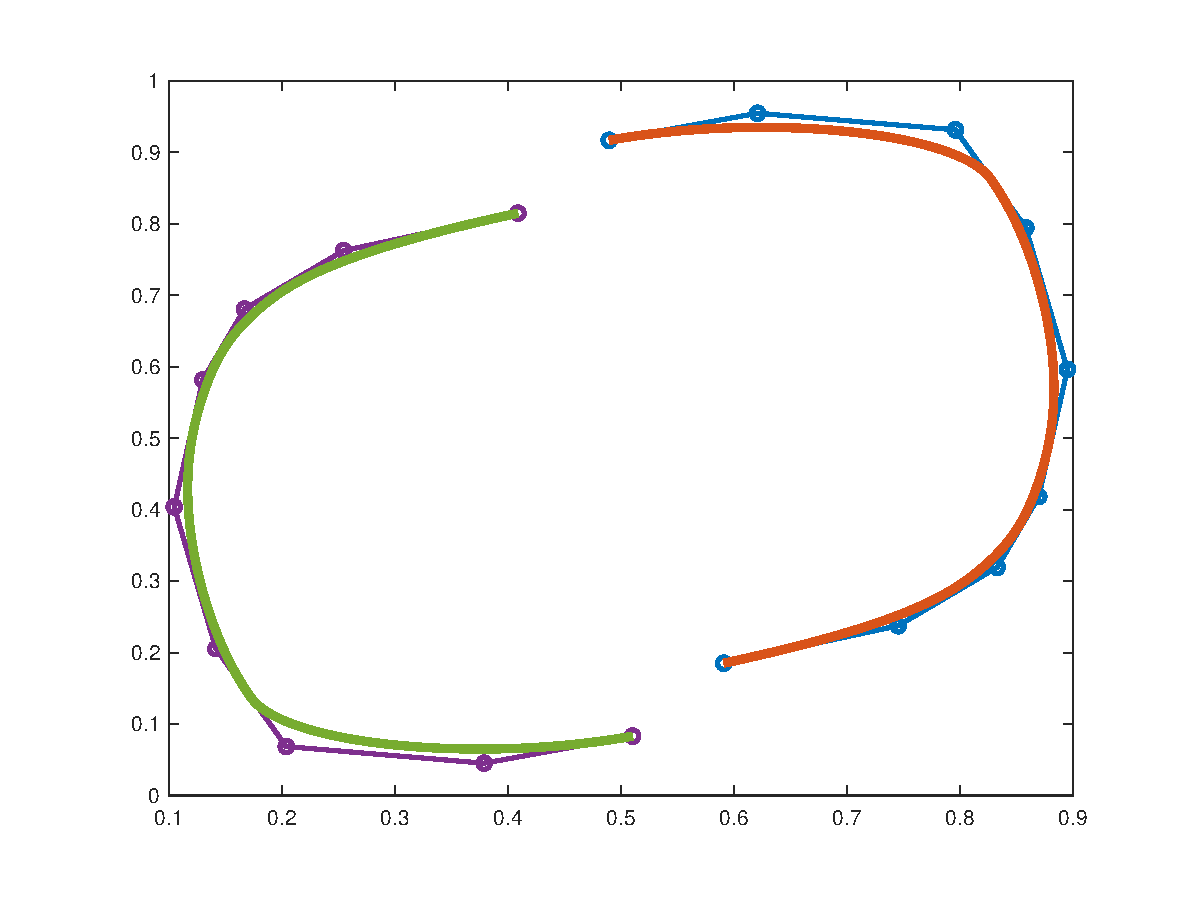
\includegraphics[width=0.75\textwidth]{figure/transformation_spline.eps}
  \caption{Trasformazione affine su spline}
  \label{fig:trasformationspline}
\end{figure} 
\lstinputlisting[label=code:trasnformationspline, firstline=2, language=Matlab, caption = Applicazone trasformazione affine]{code/b_spline_curve_prop_trans.m}



\paragraph{Località} La proprietà di località ci dice  che il punto di controllo $\mathbf{d_j}$ influenza la curva solamente per $t \in [t_j, t_{j+k}]$. 
Ad esempio, come mostrato in Figura~\ref{fig:loc_spline1} ed in Codice~\ref{code:locspline}, spostando $\mathbf{d}_7$ la curva varia da $t \in [t_7, t_{11}]$. 


\begin{figure}[]
  \centering
  \begin{subfigure}[b]{0.3\textwidth}
    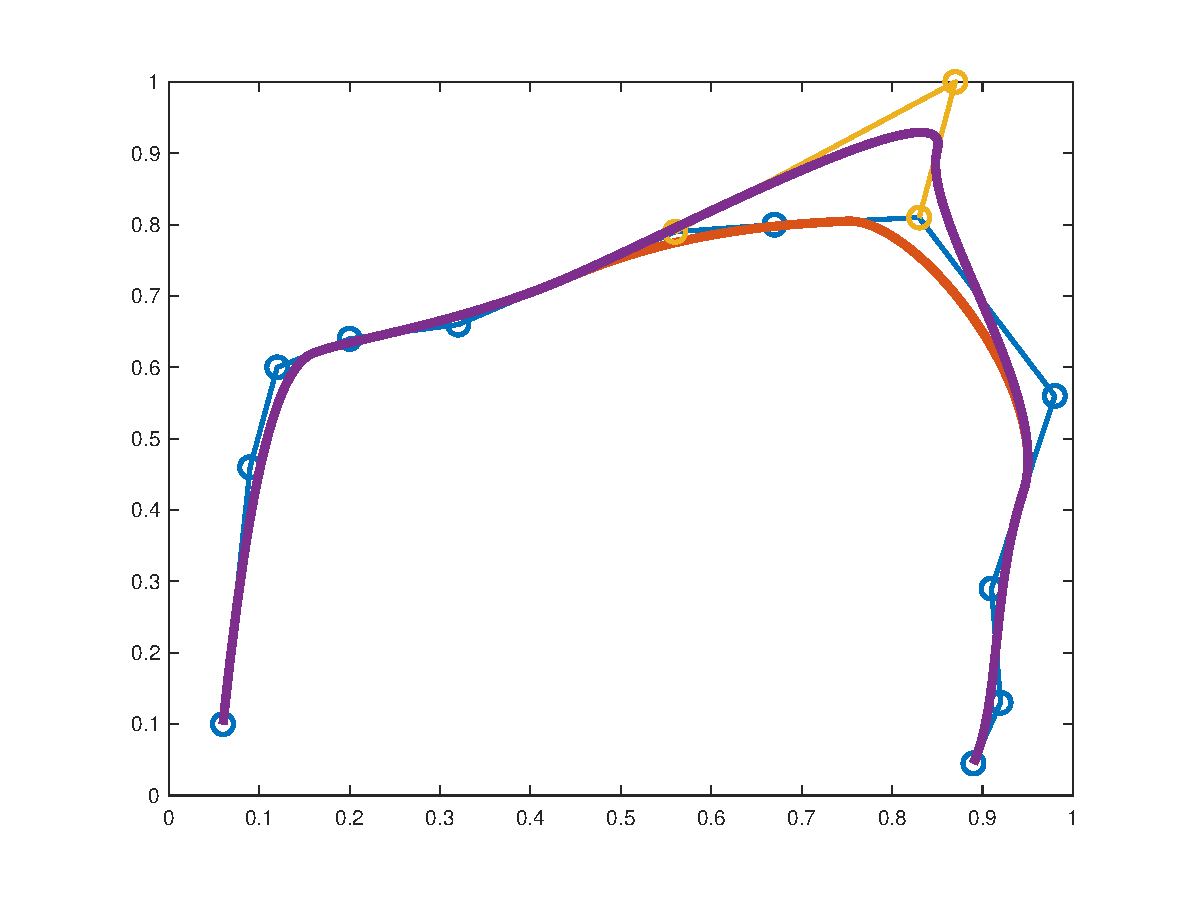
\includegraphics[width=\textwidth]{figure/loc3.eps}
    \caption{Spostamento di $\mathbf{d_7}$ }
    \label{fig:loc3}
  \end{subfigure}
  \begin{subfigure}[b]{0.3\textwidth}
      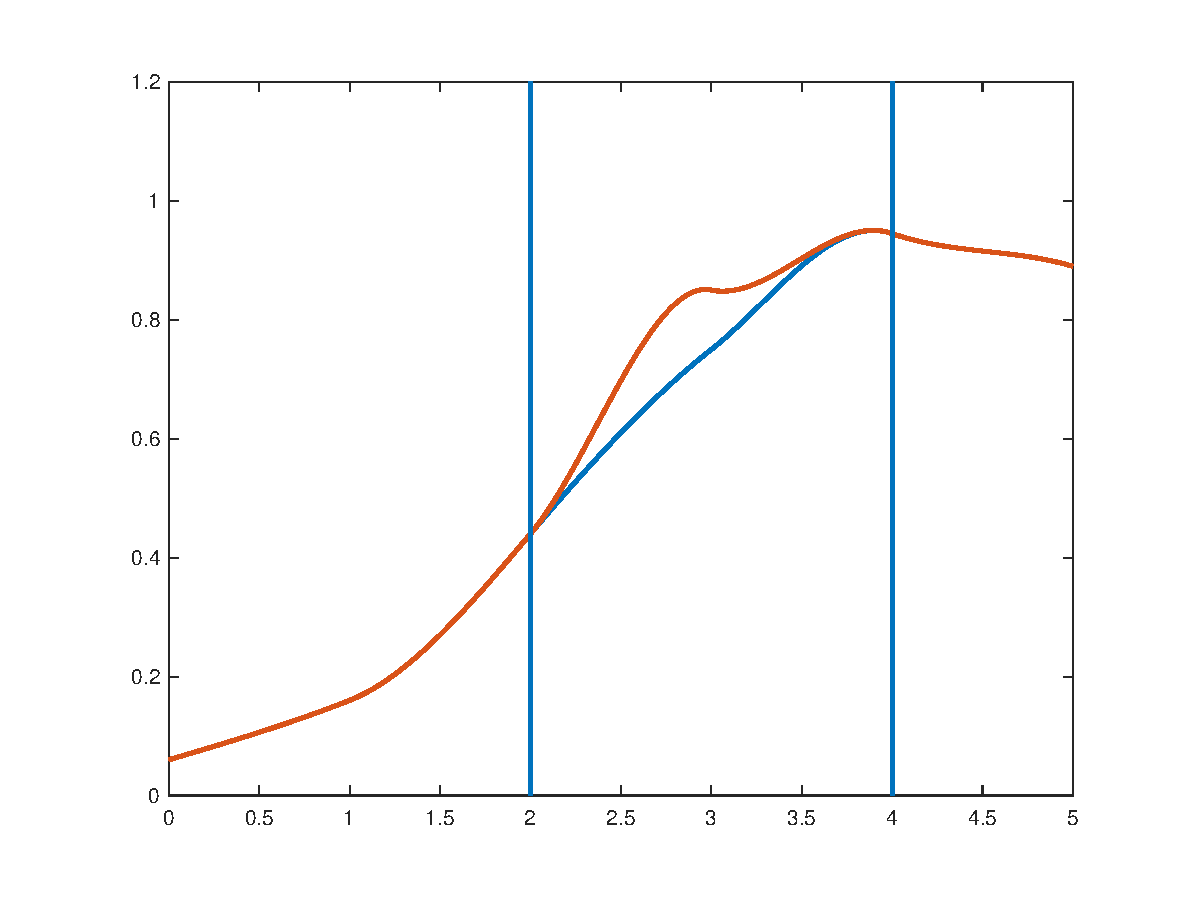
\includegraphics[width=\textwidth]{figure/loc2.eps}
      \caption{Variazione sulla $x$}
      \label{fig:loc2}
  \end{subfigure}
  \begin{subfigure}[b]{0.3\textwidth}
      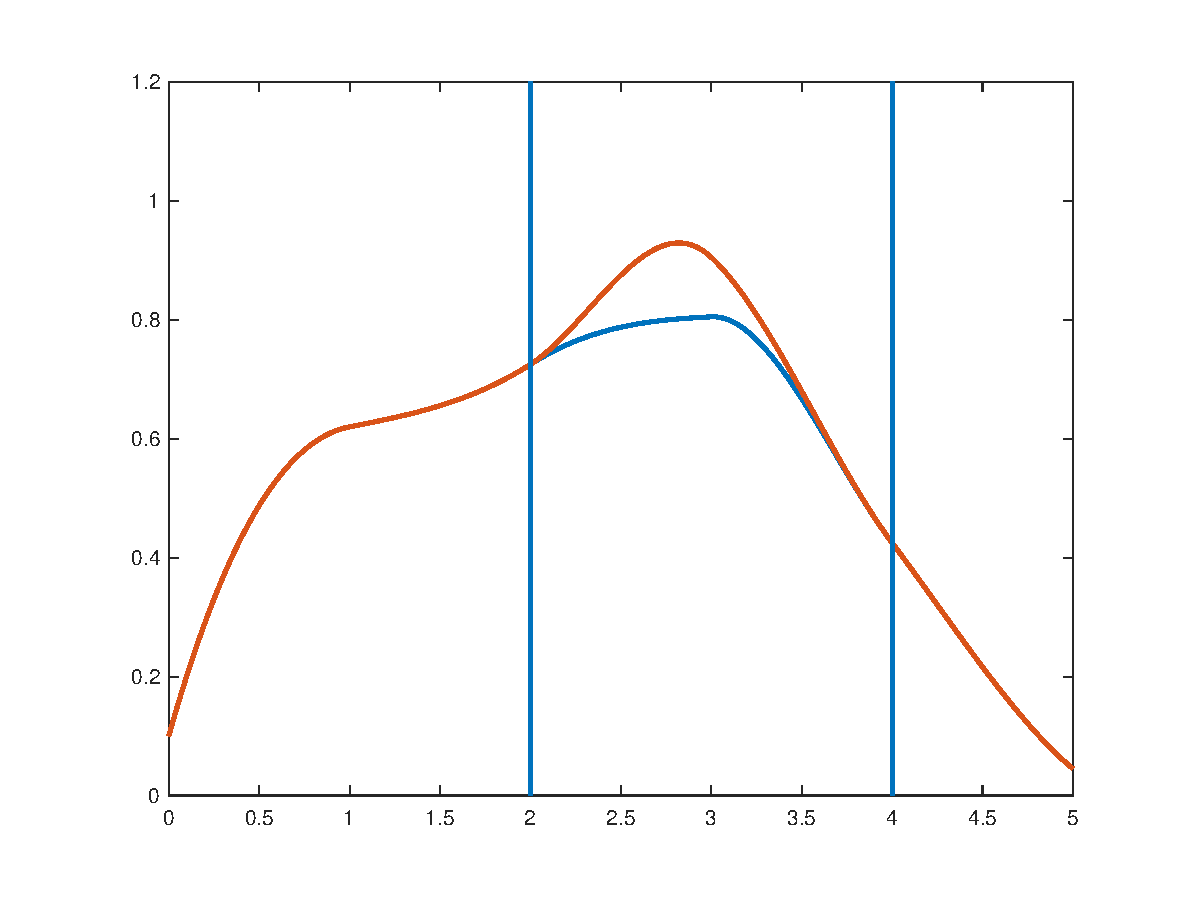
\includegraphics[width=\textwidth]{figure/loc1.eps}
      \caption{Variazione sulla $y$}
      \label{fig:loc1}
  \end{subfigure}
  \caption{Proprietà di località}\label{fig:loc_spline1}
\end{figure}
\lstinputlisting[label=code:locspline, firstline=2, lastline = 33, language=Matlab, caption = Proprietà di località]{code/b_spline_curve_prop_loc.m}
La proprietà di località ci dice anche che una curva \textit{B-Spline} $\mathbf{X}(t^*)$ con $t^* \in [t_r, t_{r+1})$ è determinata da 
$k$ punti di controllo $d_{r-k+1}, \dots, d_{r}$. 
Utilizzando Codice~\ref{code:locspline1} viene mostrata questa proprietà. Per questo esempio è stato scelto
$r = 8$, ed una partizione nodale mostrata a Riga 2 del Codice~\ref{code:locspline}.
I  punti di controllo spostati sono $8$, ovvero i $\mathbf{d}_j \notin [\mathbf{d}_{5}, \mathbf{d}_{8}]$.
Come mostrato in Figura~\ref{fig:loc_spline1} la curva  $\mathbf{X}(t^*)$  rimane quindi invariata per $t^* \in [t_{8}, t_{9})$. 

\lstinputlisting[label=code:locspline1, firstline=36, language=Matlab, caption = Proprietà di località]{code/b_spline_curve_prop_loc.m}



\begin{figure}[]
  \centering
  \begin{subfigure}[b]{0.3\textwidth}
    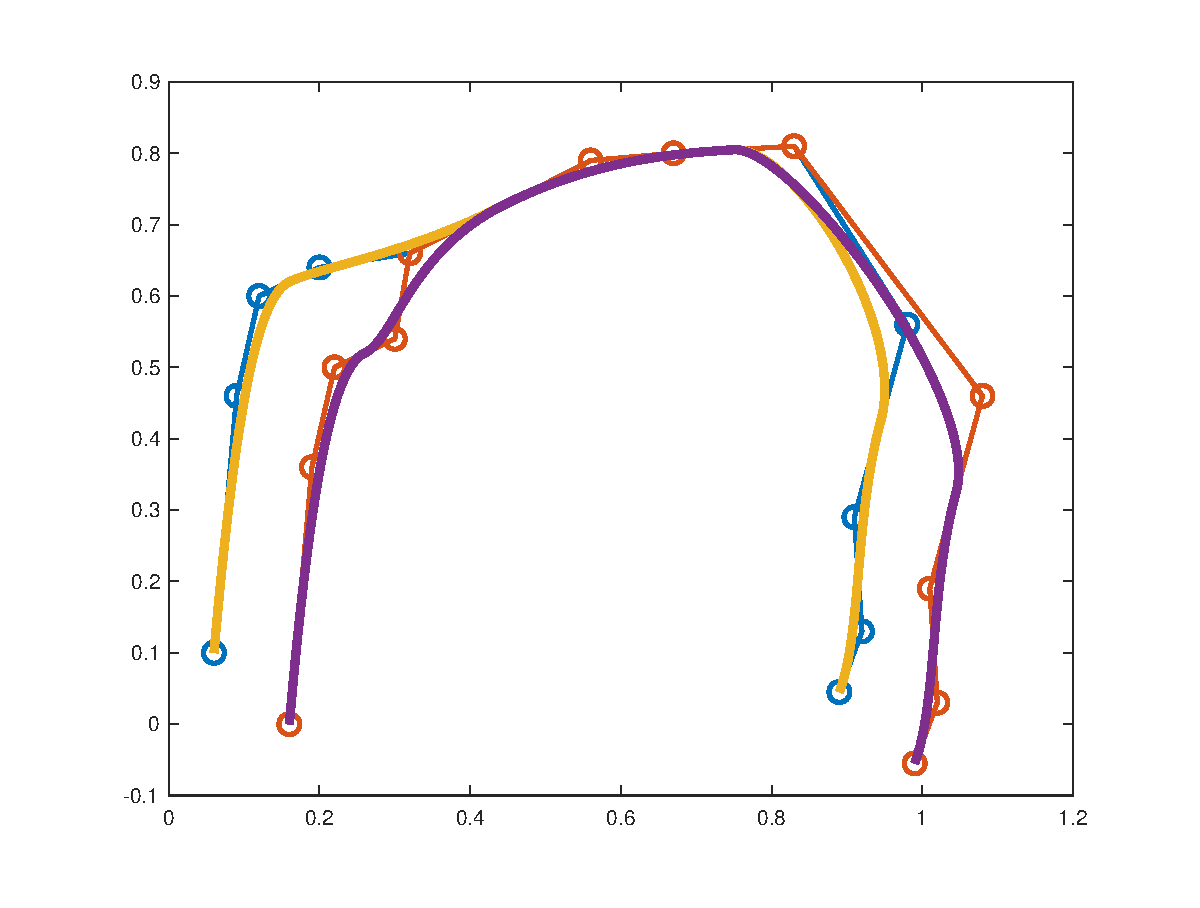
\includegraphics[width=\textwidth]{figure/loc6.eps}
    \caption{Spostamento di $\mathbf{d}_j \notin [\mathbf{d}_{5}, \mathbf{d}_{8}]$ }
    \label{fig:loc6}
  \end{subfigure}
  \begin{subfigure}[b]{0.3\textwidth}
      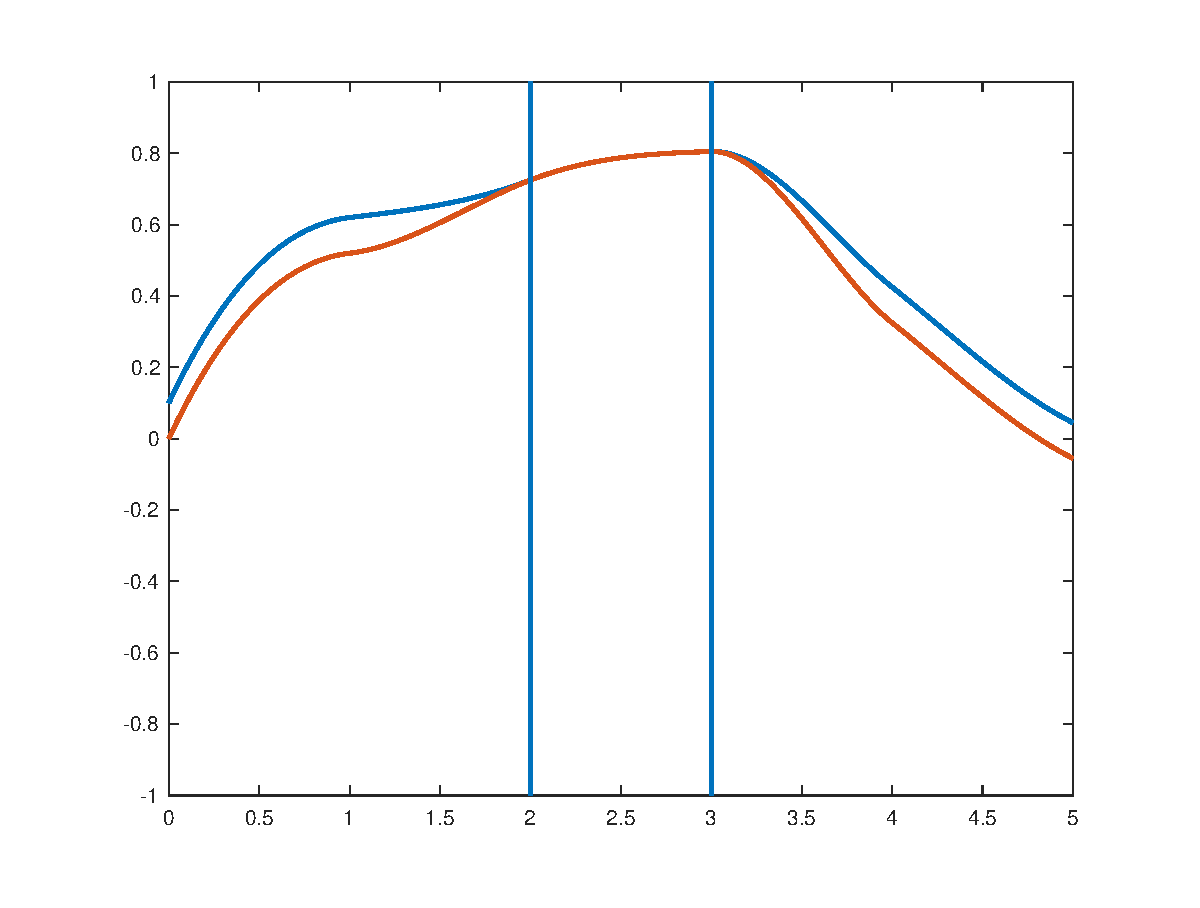
\includegraphics[width=\textwidth]{figure/loc5.eps}
      \caption{Variazione sulla $x$}
      \label{fig:loc5}
  \end{subfigure}
  \begin{subfigure}[b]{0.3\textwidth}
      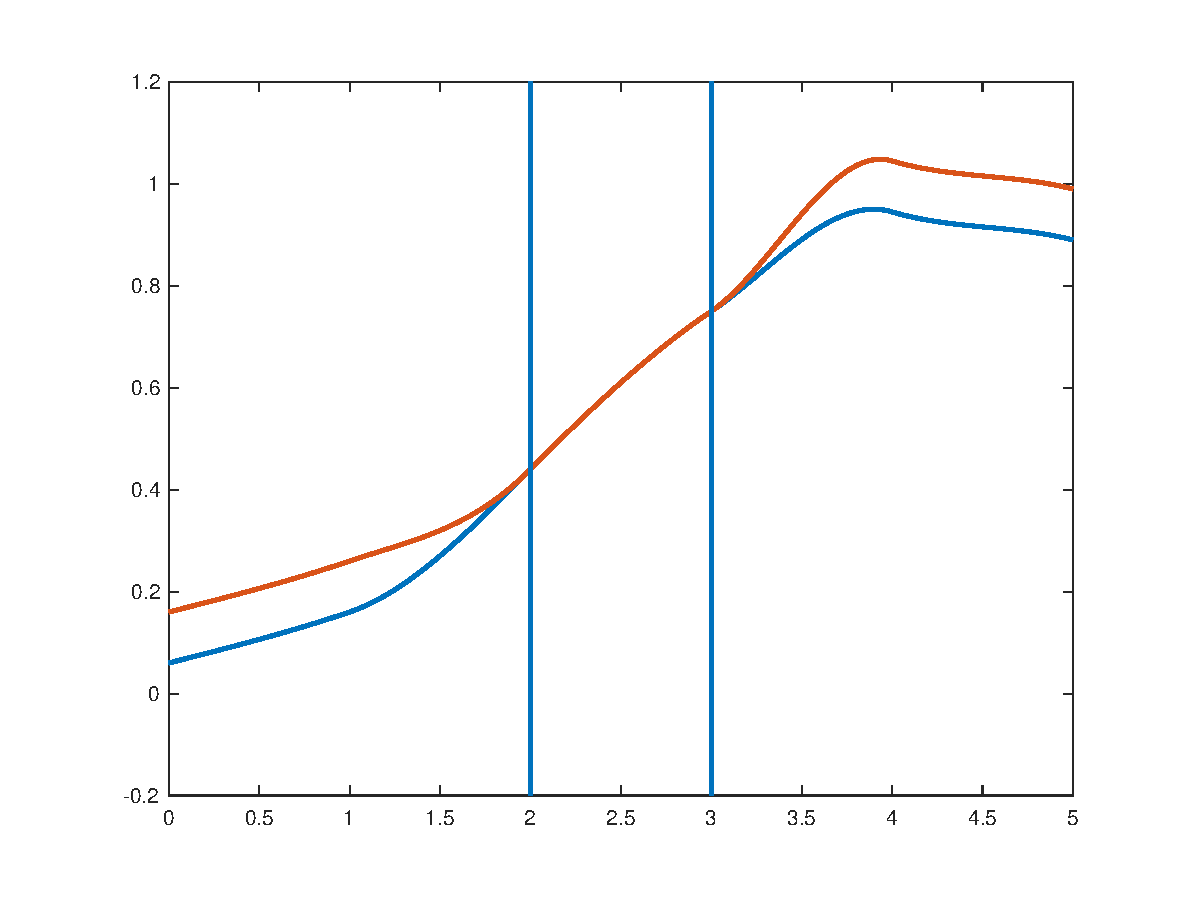
\includegraphics[width=\textwidth]{figure/loc4.eps}
      \caption{Variazione sulla $y$}
      \label{fig:loc4}
  \end{subfigure}
  \label{fig:loc_spline}
\end{figure} 



\paragraph{Variation Diminishing}
La proprietà di Variation Diminishing dice che presa una qualunque retta che interseca
un numero $b$ di volte il poligono di controllo, questa intersecherà un numero di volte $a \leq b$ la curva \textit{B-Spline} 
disegnata a partire dal poligono di controllo. 
Un esempio realizzato con il Codice~\ref{code:vardim} è mostrato in Figura~\ref{fig:intersection}.
\lstinputlisting[label=code:vardim, firstline=2, language=Matlab, caption = Proprietà di Variation Diminishing]{code/b_spline_curve_prop_var_dim.m}
\begin{figure}[]
  \centering
  \begin{subfigure}[b]{0.3\textwidth}
    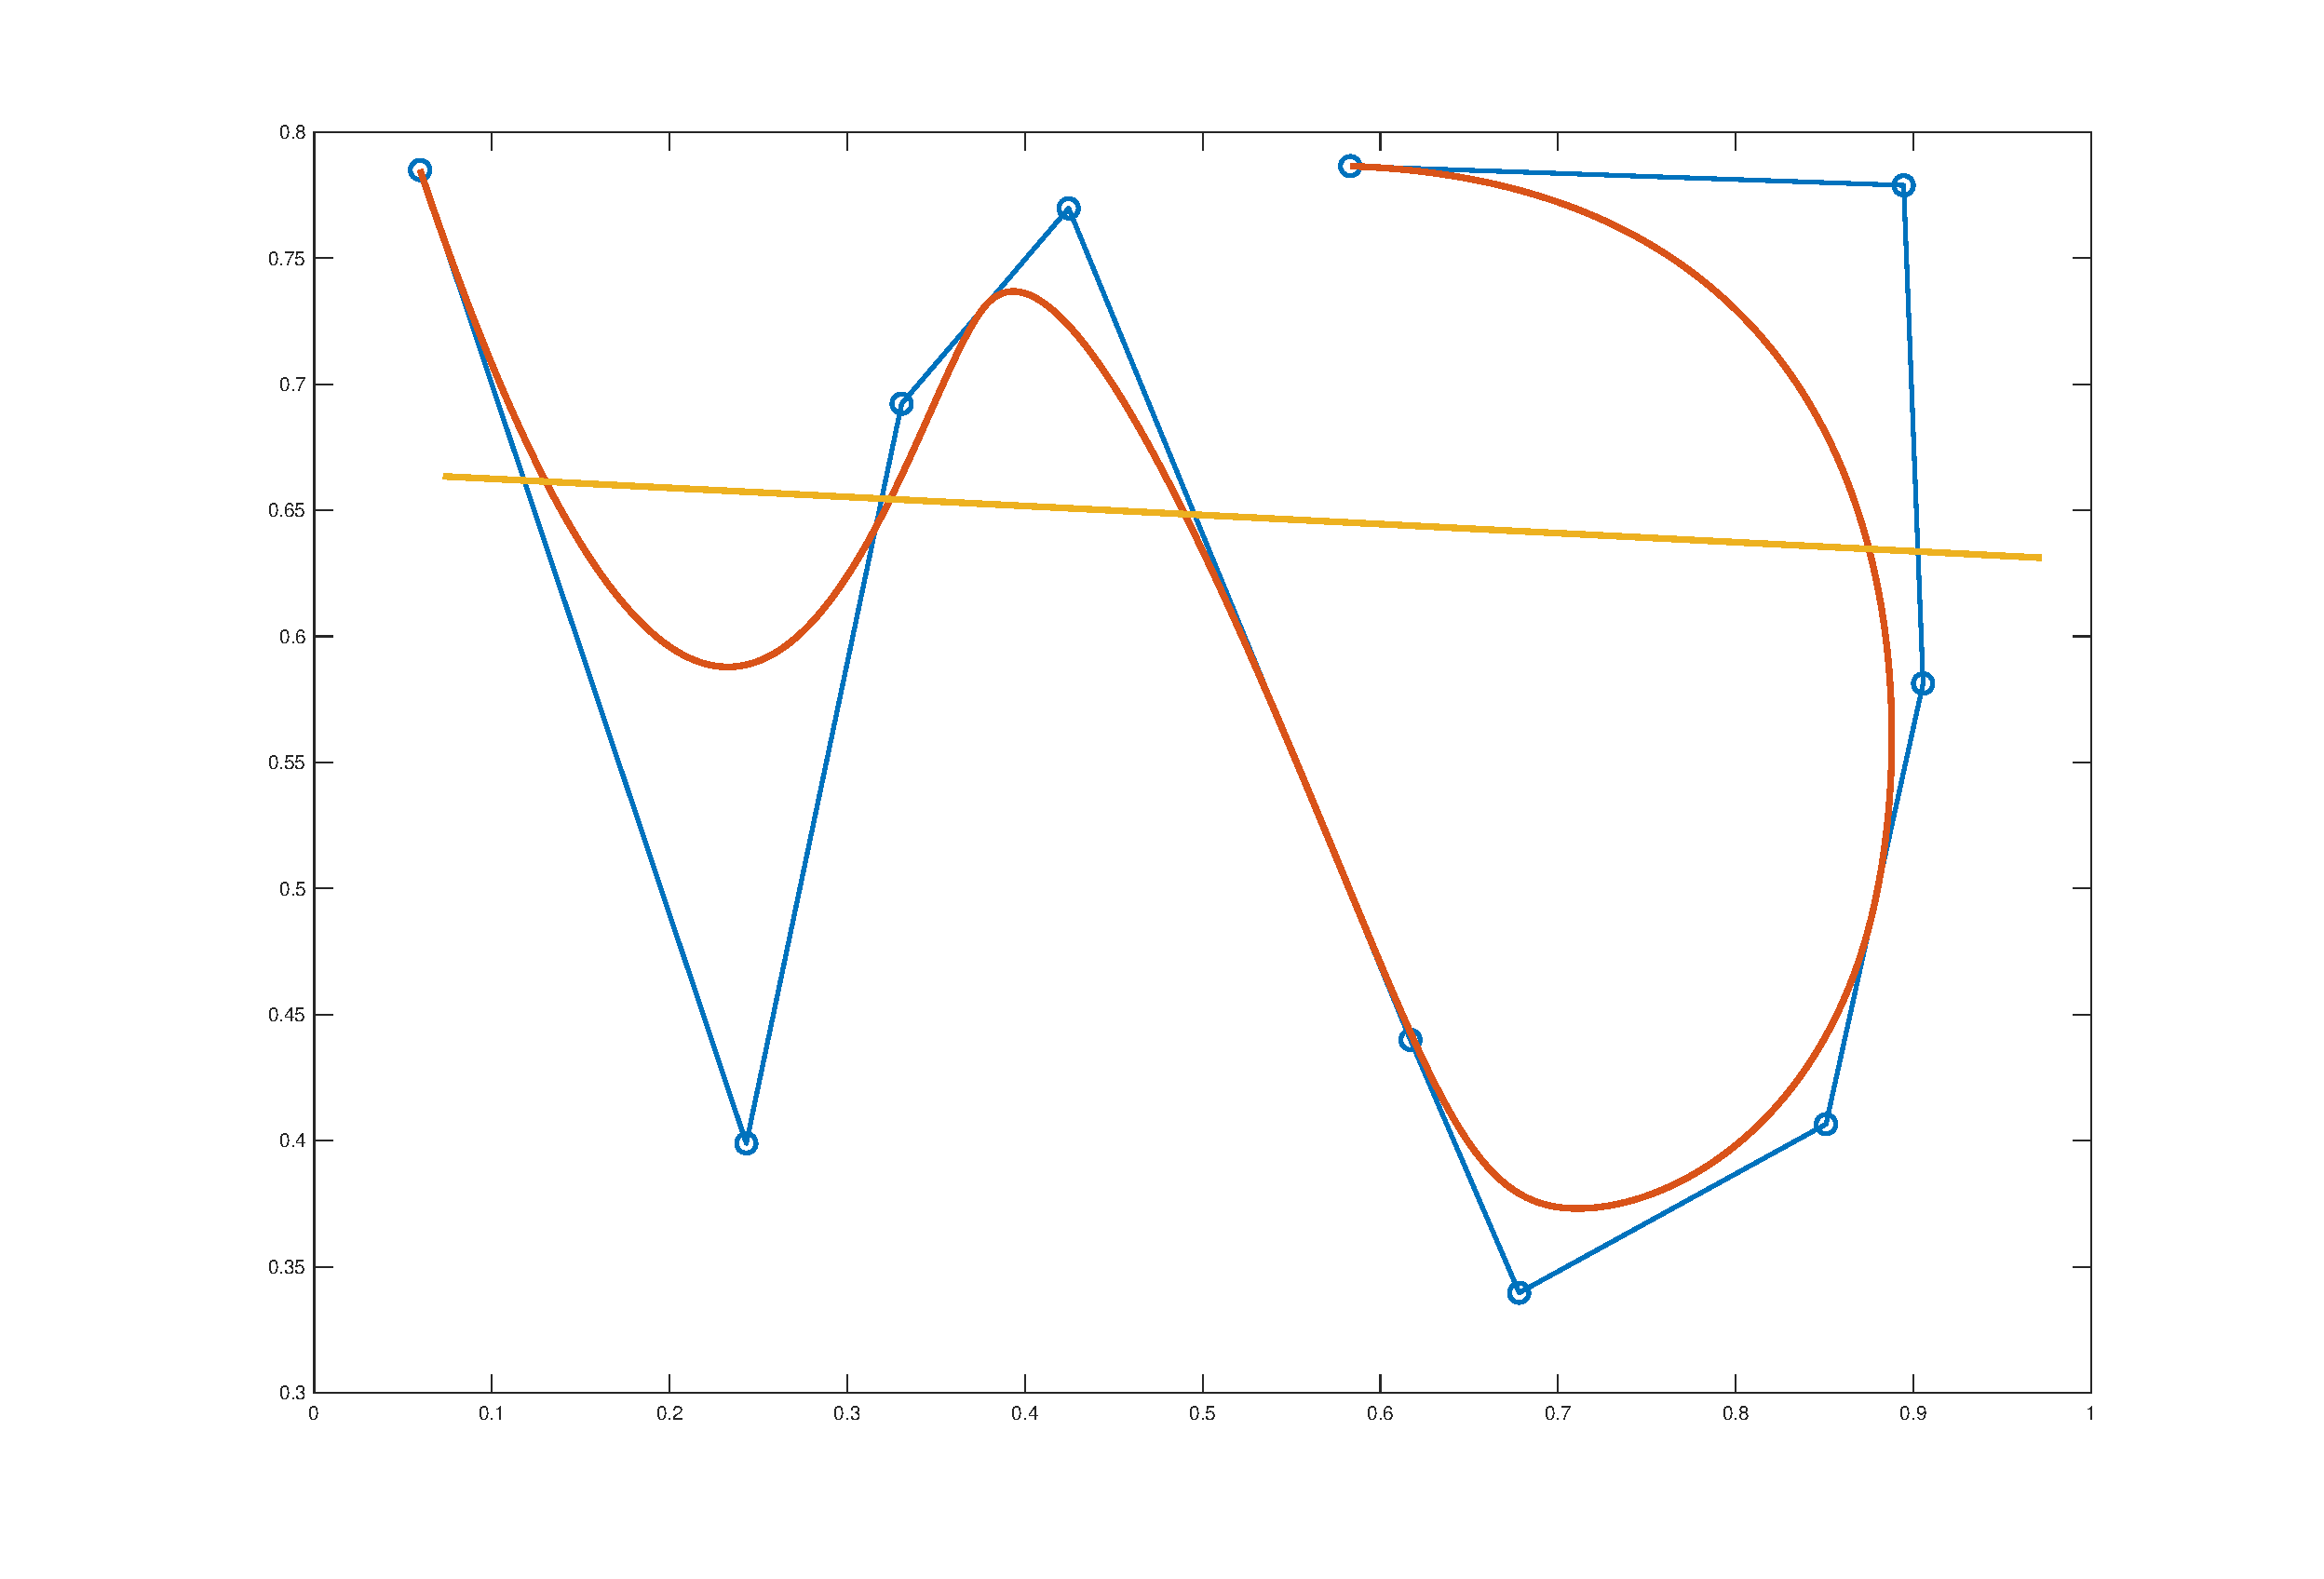
\includegraphics[width=\textwidth]{figure/intersection1.eps}
    \caption{Poligono: $4$, Curva: $4$}
    \label{fig:intersection1}
  \end{subfigure}
  \begin{subfigure}[b]{0.3\textwidth}
      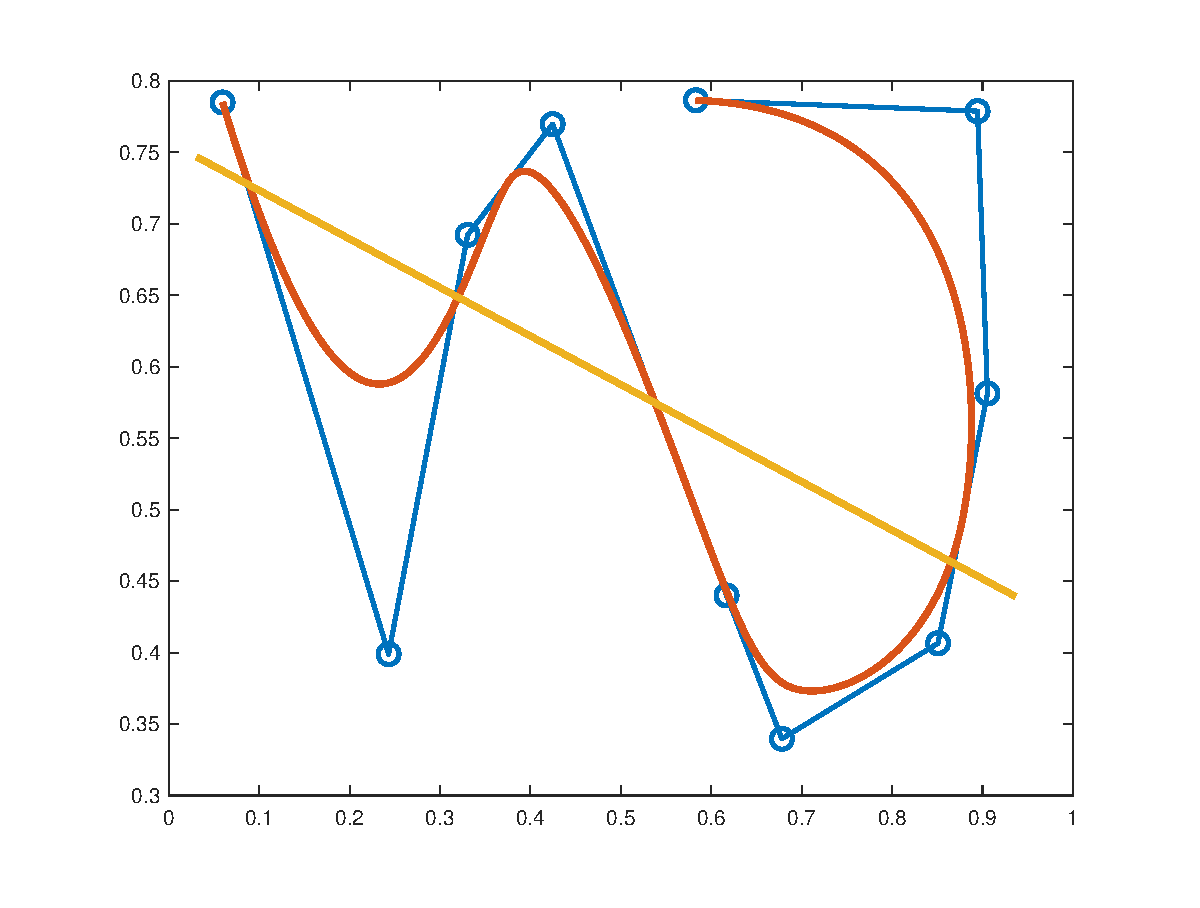
\includegraphics[width=\textwidth]{figure/intersection3.eps}
      \caption{Poligono: $4$, Curva: $4$}
      \label{fig:intersection3}
  \end{subfigure}
  \begin{subfigure}[b]{0.3\textwidth}
      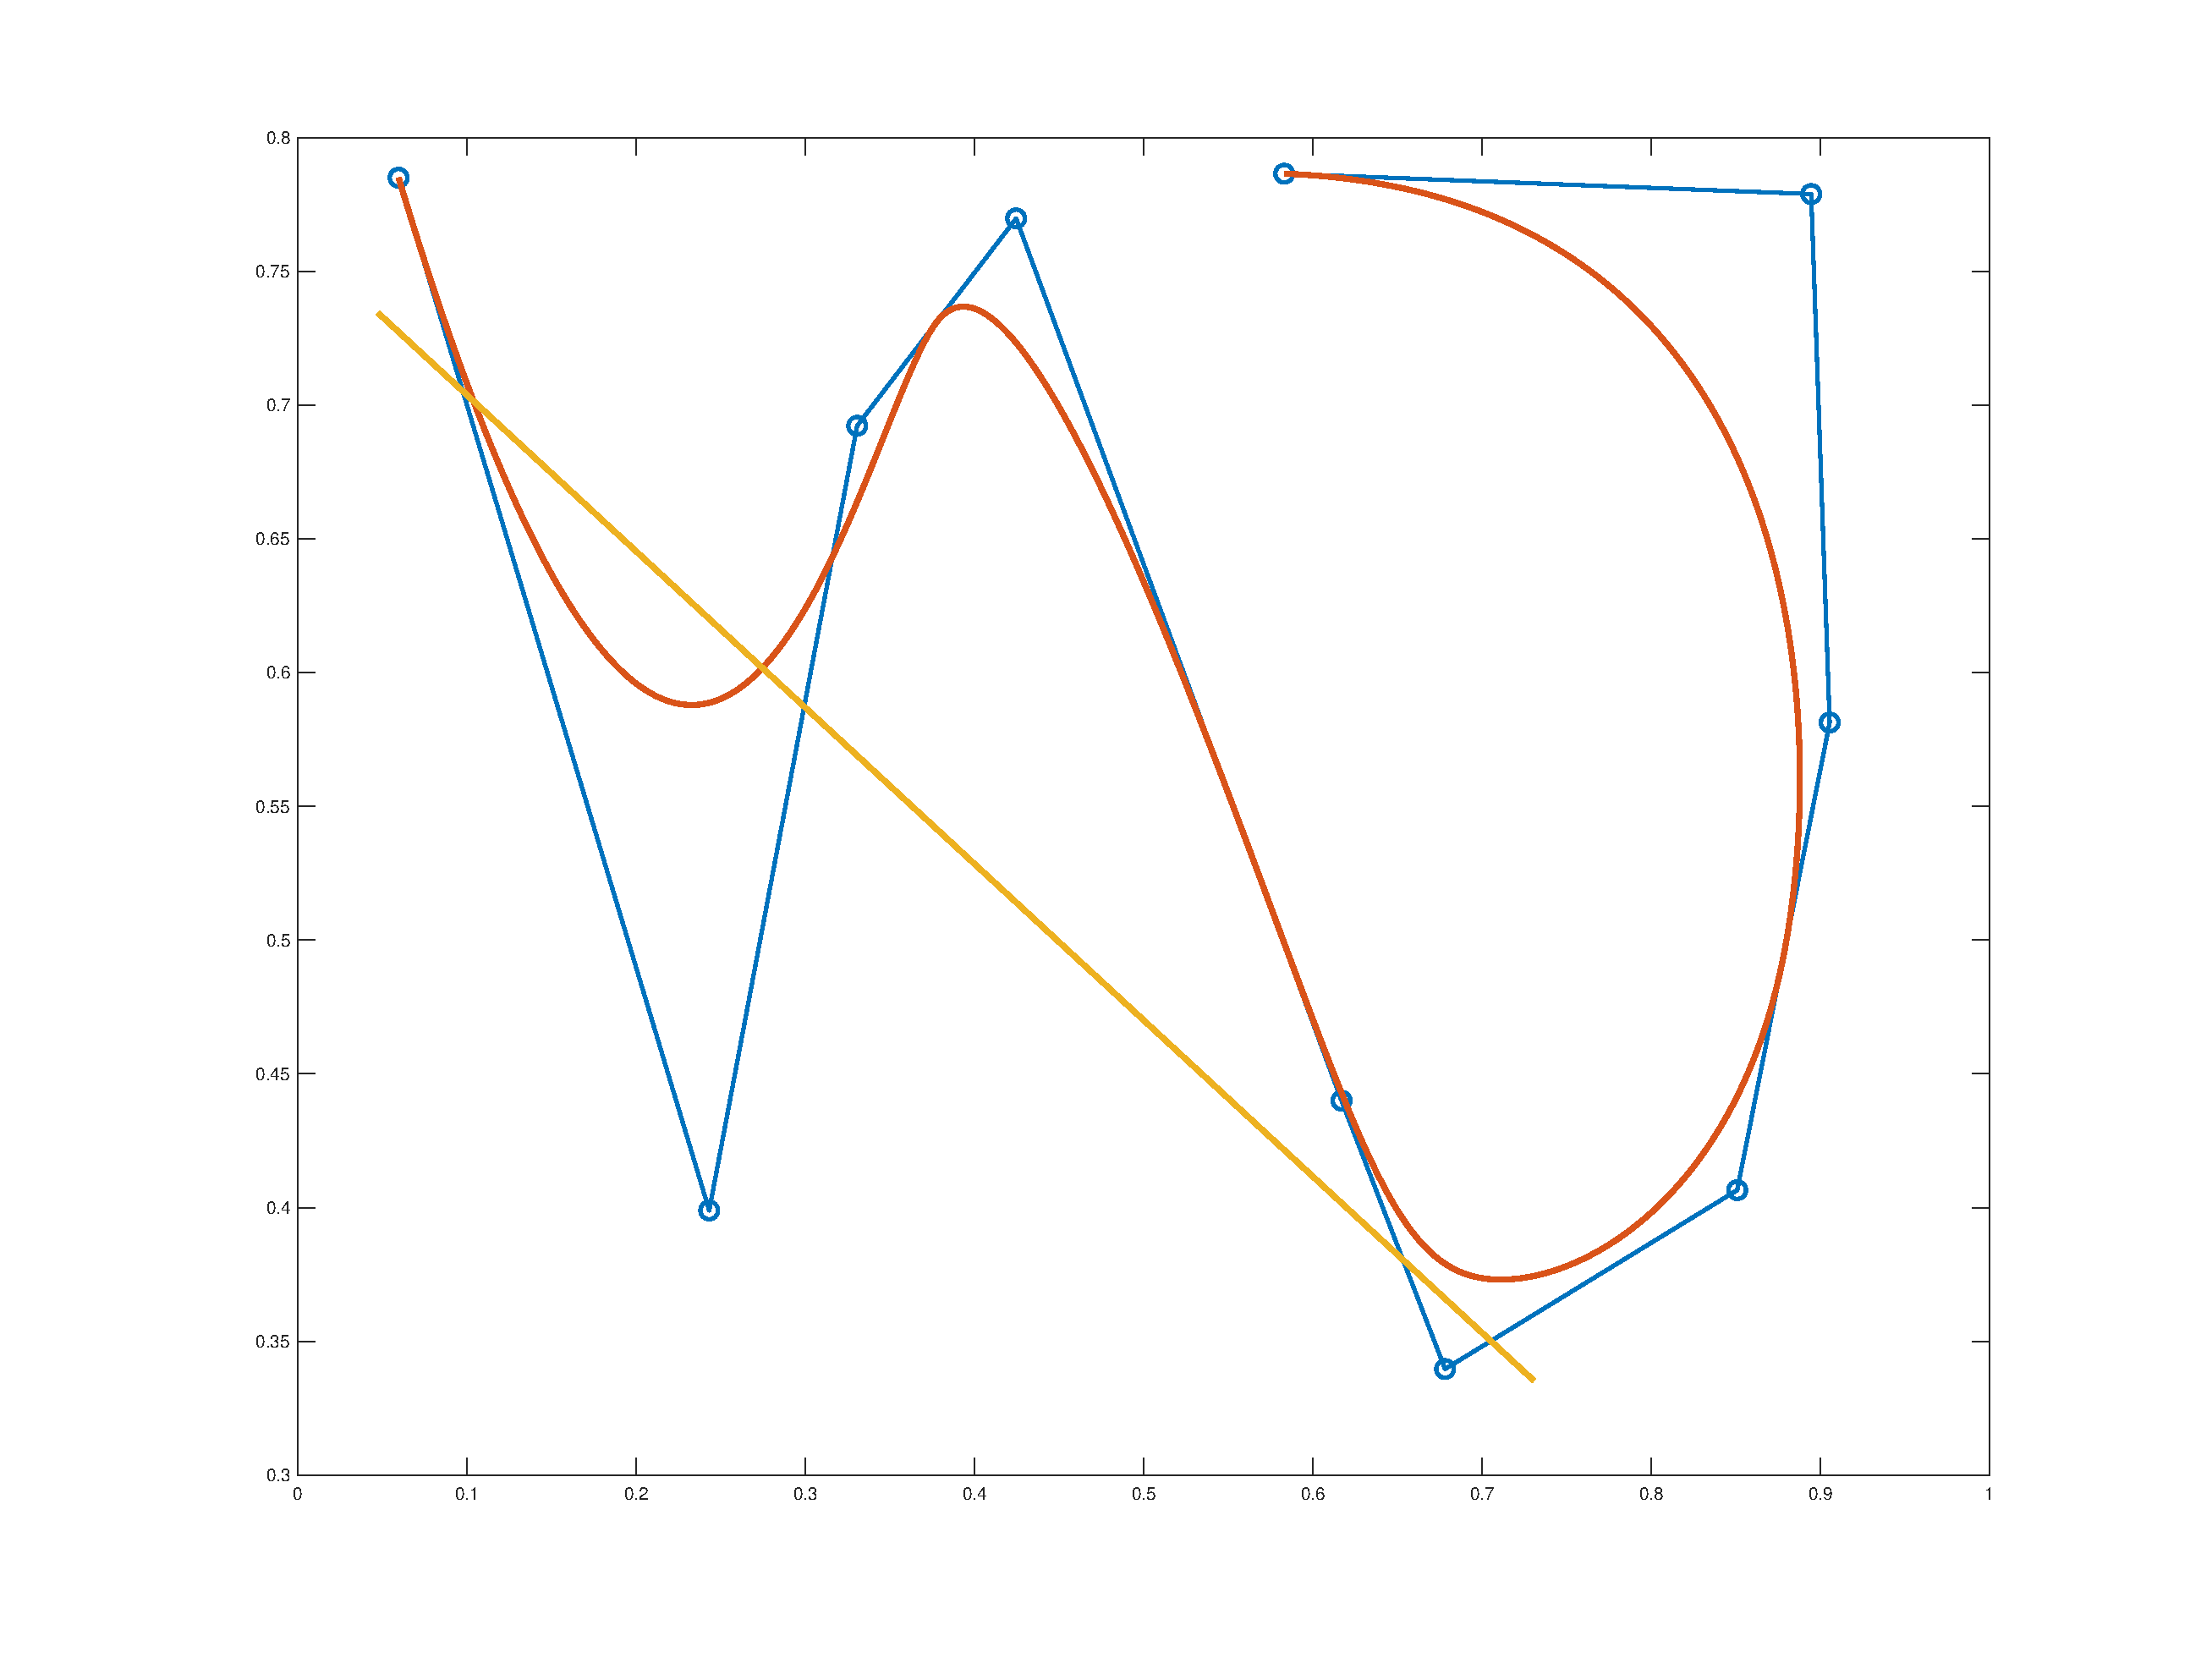
\includegraphics[width=\textwidth]{figure/intersection4.eps}
      \caption{Poligono: $4$, Curva: $2$}
      \label{fig:intersection4}
  \end{subfigure}
  \begin{subfigure}[b]{0.3\textwidth}
    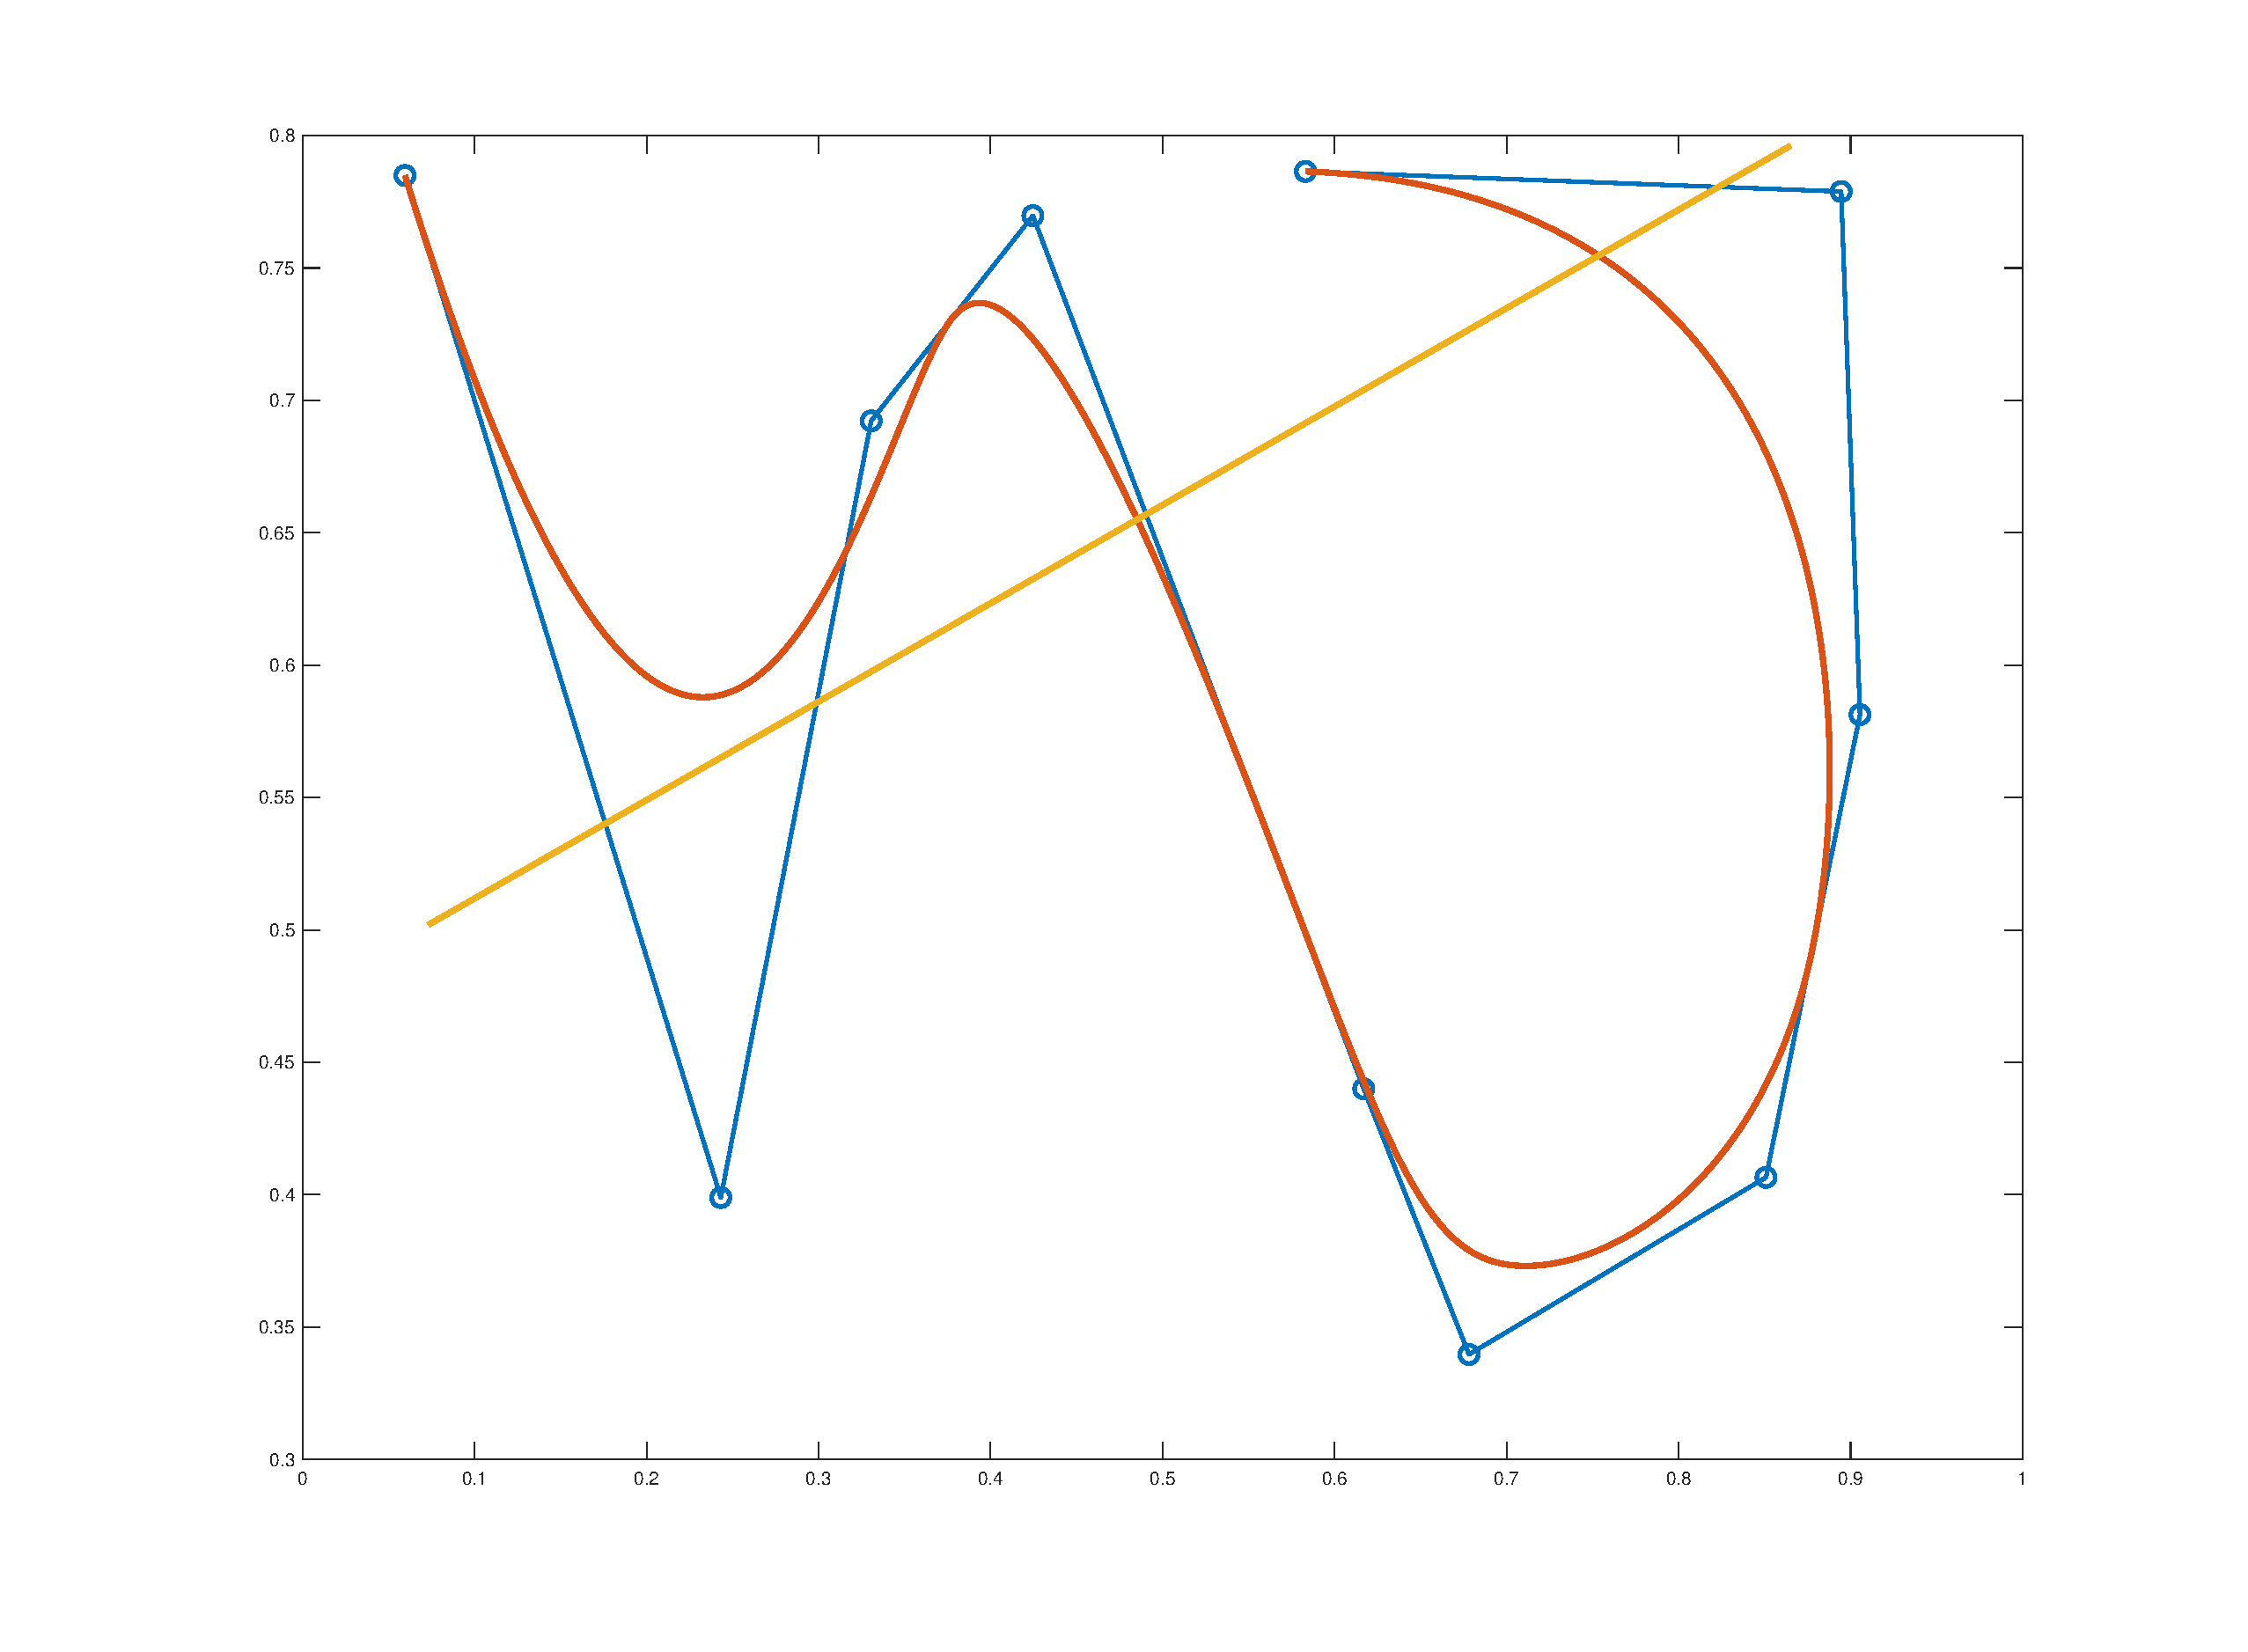
\includegraphics[width=\textwidth]{figure/intersection5.eps}
    \caption{Poligono: $4$, Curva: $2$}
    \label{fig:intersection5}
  \end{subfigure}
  \caption{Proprietà di Variation Diminishing}\label{fig:intersection}
\end{figure}
\subsection{Continuità}
Consideriamo due curve di \textit{Bézier} (che ricordiamo essere un caso particolare di curve \textit{B-Spline}) $C_1(u)$ e $C_2(v)$, definite rispettivamente su $u \in [u_a, u_b]$ e $v \in [v_a, v_b]$ e sui
vertici di controllo $\{\mathbf{V}_{1,1},\dots, \mathbf{V}_{n,1}\}$ e $\{\mathbf{V}_{1,2},\dots, \mathbf{V}_{m,2}\}$. 
Consideriamo ora il caso in cui queste due curve si uniscono, usando come punto di raccordo l'ultimo vertice della prima curva
ed il primo vertice della seconda curva. Possono verificarsi diversi casi descritti di seguito. 
Per generare le Figure~\ref{fig:discontinuity}, ~\ref{fig:continuityc0},  ~\ref{fig:continuityc1} e ~\ref{fig:continuityg1}, mostrate in seguito, è stato usato il Codice~\ref{code:continuity}.
\lstinputlisting[label=code:continuity, firstline=2, language=Matlab, caption = Continuità sulle curve]{code/b_spline_curve_prop_var_dim.m}

\paragraph{Discontinuità}
Il primo caso è la discontinuità chiamata, con abuso di notazione, $C^{-1}$. Questa si verifica
quando l'ultimo vertice della prima curva è diverso dal primo vertice della seconda curva, ovvero:
$$V_{n,1} \neq V_{0, 2}$$
Un esempio è possibile vederlo in Figura~\ref{fig:discontinuity}.
\begin{figure}[]
  \centering
  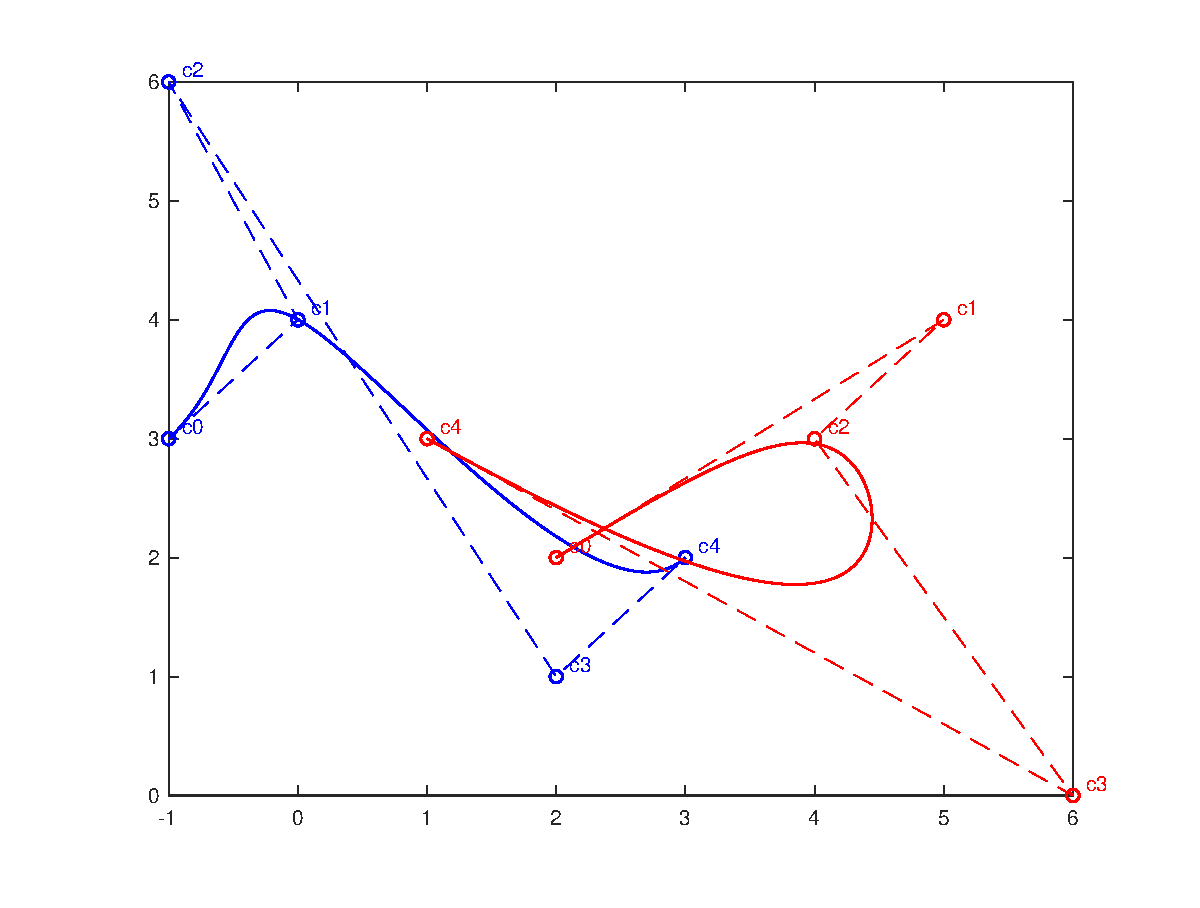
\includegraphics[width=0.75\textwidth]{figure/discontinuity.eps}
  \caption{Curve discontinue}
  \label{fig:discontinuity}
\end{figure} 

\paragraph{Continuità $C^0$}
Date due curve la condizione per far sì che ci sia continuità di tipo $C^0$ è che 
l'ultimo vertice della prima curva coincida con il primo vertice della seconda curva, ovvero che:
$$\mathbf{V}_{n,1} = \mathbf{V}_{1, 2}$$
Un esempio di tale continuità è presente in Figura~\ref{fig:continuityc0}
\begin{figure}[]
  \centering
  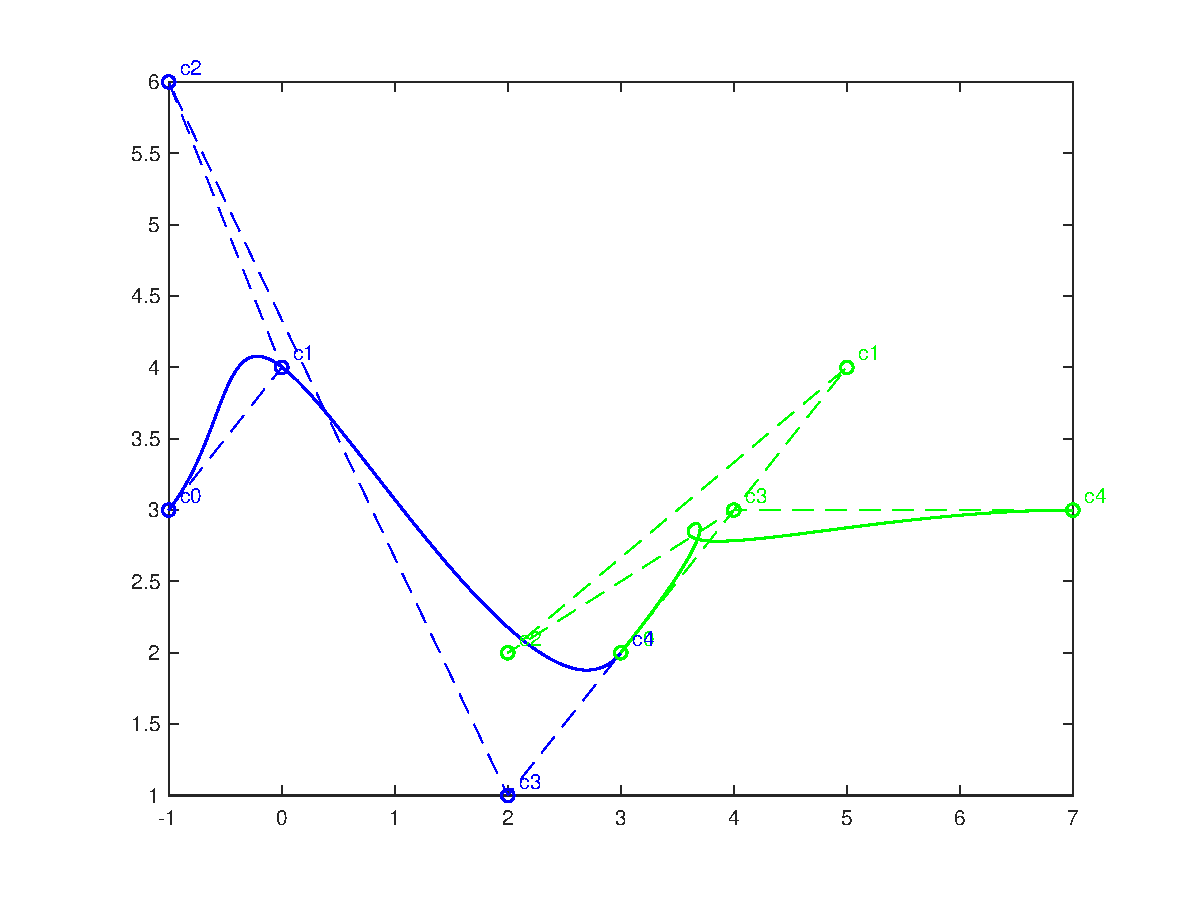
\includegraphics[width=0.75\textwidth]{figure/continuity_c0.eps}
  \caption{Continuità $C^0$}
  \label{fig:continuityc0}
\end{figure} 

\paragraph{Continuità $C^1$}
La continuità $C^1$ si impone con la seguente condizione sulla derivata prima:
$$C'_1(\mathbf{V}_{n, 1}) = C'_2(\mathbf{V}_{1, 2})$$
Per far sì che questa condizione sia verificata è sufficiente posizionare il 
penultimo vertice della prima curva, il secondo della seconda curva ed il punto di giunzione per la continuità $C^0$ sulla stessa retta.
Analiticamente ciò vuol dire imporre la seguente ugualianza:
$$\mathbf{V}_{2,2} = 2\mathbf{V}_{n, 1} - \mathbf{V}_{n-1, 1}$$
\begin{figure}[]
  \centering
  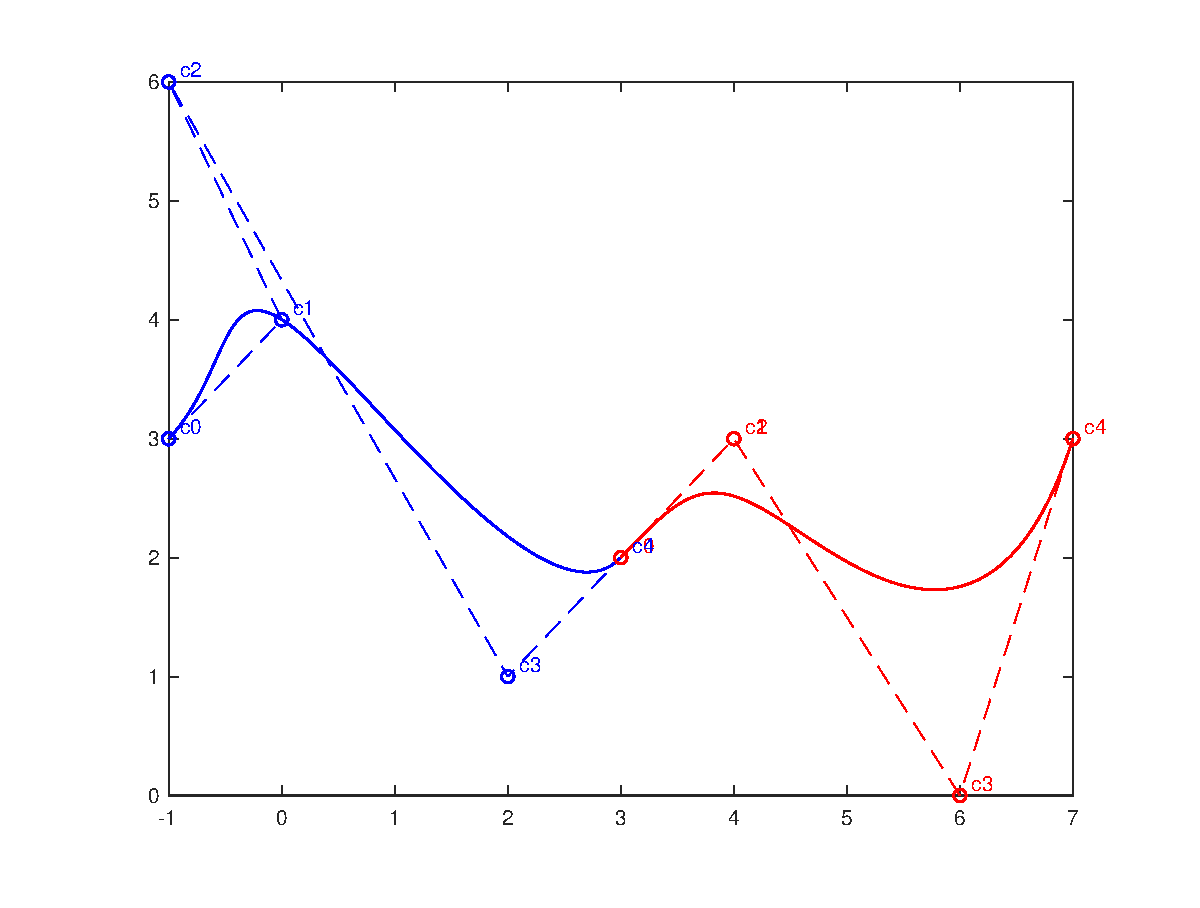
\includegraphics[width=0.75\textwidth]{figure/continuity_c1.eps}
  \caption{Continuità $C^1$}
  \label{fig:continuityc1}
\end{figure} 
Un esempio è mostrato in Figura~\ref{fig:continuityc1}.

\paragraph{Continuità $G^1$}
La continuità $G^1$ è un particolare tipo di continuità chiamata anche \textit{Continuità geometrica}. Questo tipo 
di continuità non dipende dalla parametrizzazione della curva. La condizione per far sì che sia presente questo 
particolare tipo di continuità è la seguente:
$$C'_2(v_0) = \omega C'_1(u_1)$$ con $\omega$ a piacere.
Un esempio di continuità $G^1$ è mostrato in Figura~\ref{fig:continuityg1}.
\begin{figure}[]
  \centering
  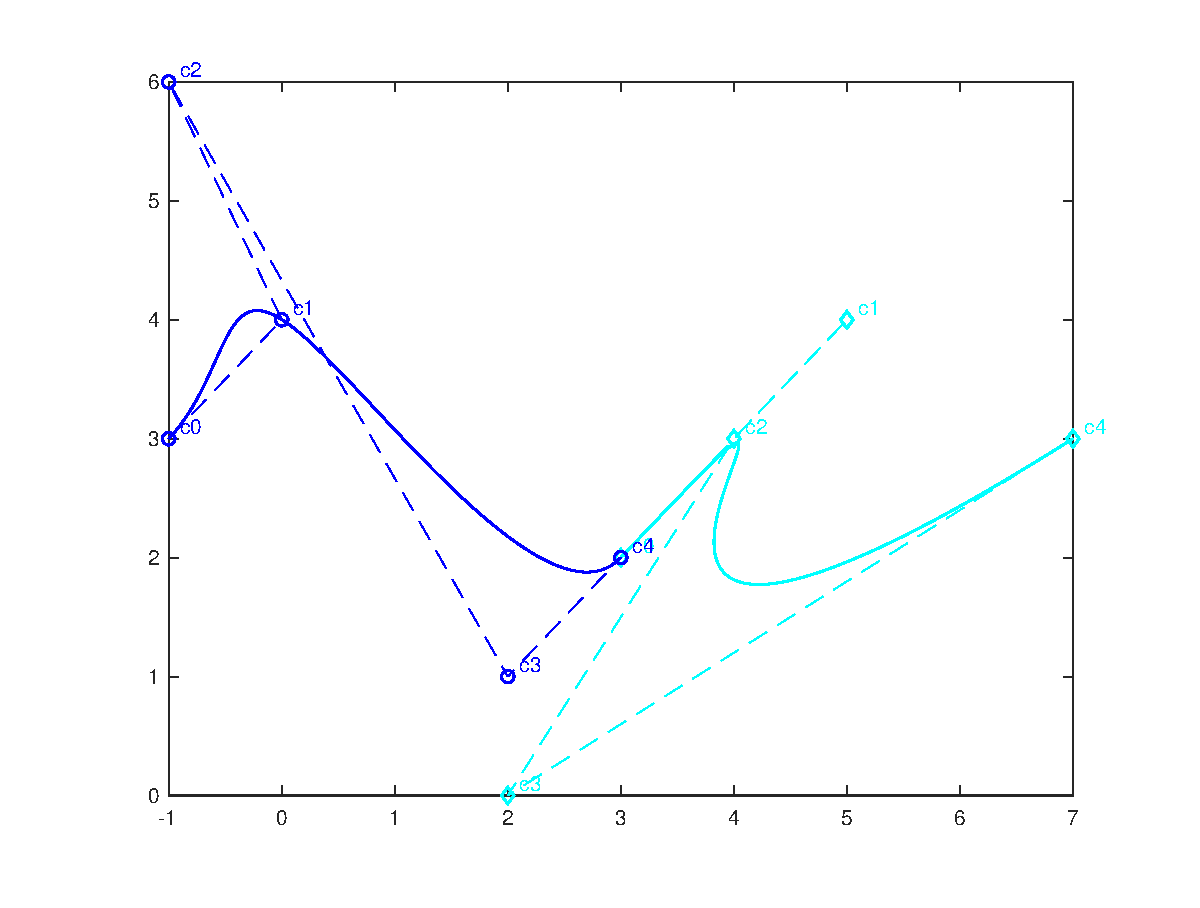
\includegraphics[width=0.75\textwidth]{figure/continuity_g1.eps}
  \caption{Continuità $G^1$}
  \label{fig:continuityg1}
\end{figure} 
\subsection{Curve Chiuse}
Grazie ai nodi ausiliari ciclici è possibile usare la base delle \textit{B-Spline} per generare
curve chiuse. In Codice~\ref{code:closed_curve} è possibile vedere un esempio di implementazione di una curva chiusa di 
ordine $k = 4$.
Per ottenere una curva con questa proprietà è necessario generare una partizione nodale estesa in questo modo:
$$\Delta^* = \left[ \underbrace{\frac{-k}{m-1}}_{Inizio} : \underbrace{\frac{1}{m-1}}_{Passo} : \underbrace{\frac{k+m-1}{m-1}}_{Fine} \right]$$
con $k$ ordine della spline e $m$ numero di vertici di controllo della curva.
Successivamente è anche necessario estendere il poligono di controllo ripetendo i primi $k-1$ vertici.
\lstinputlisting[label=code:closed_curve, firstline=2, language=Matlab, caption = Curva chiusa]{code/b_spline_curve.m}
\begin{figure}[]
  \centering
  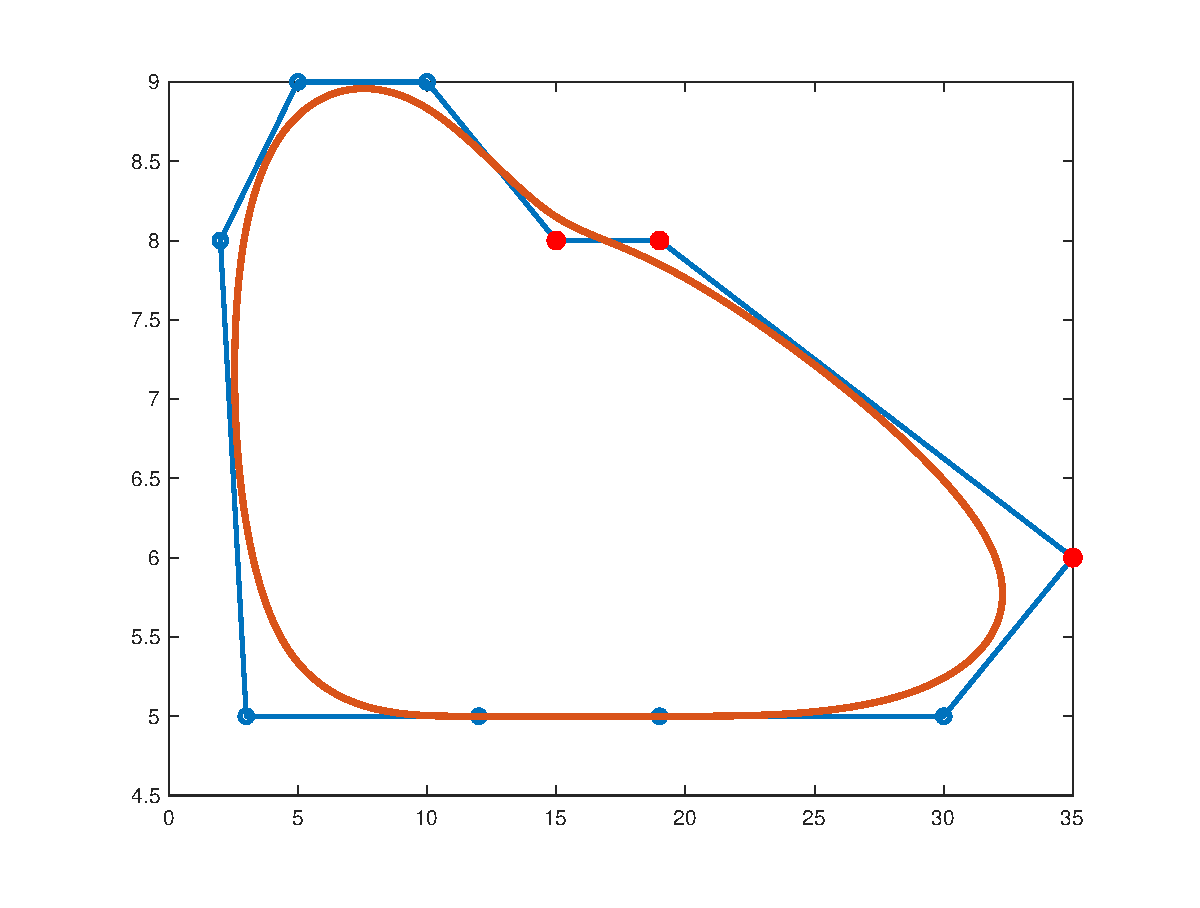
\includegraphics[width=0.75\textwidth]{figure/closed_curve.eps}
  \caption{Curva chiusa (in rosso i vertici ripetuti)}
  \label{fig:closed_curve}
\end{figure} 
In Figura~\ref{fig:closed_curve} è possibile vedere il risultato del Codice~\ref{code:closed_curve}, i vertici di controllo rossi sono 
quelli ripetuti.

\subsection{Interpolazione}

L'interpolazione consiste nel far passare la curva per un determinato insieme di punti $\mathbf{p}_1, \dots, \mathbf{p}_n$.
Dopo aver scelto adeguatamente la partizione nodale è necessario generare la base per le \textit{B-Spline}. Successivamente 
bisogna trovare i punti di controllo per generare la curva interpolante. 
Per trovare i punti di controllo della curva interpolante è necessario risolvere il seguente sistema lineare:
$$N \cdot Coefs = P$$
con $N$ base delle \textit{B-Spline} e $P$ punti di interpolazione. Nella risoluzione di tale sistema bisogna stare 
attenti a produrre una matrice $N$ \textit{non singolare}.
Il Codice~\ref{code:interpolation} genera due splines interpolanti mostrate in Figura~\ref{fig:interpolation}. I punti in rosso sono i   
$\mathbf{p}_1, \dots, \mathbf{p}_n$ di interpolazione, mentre 
rispettivamente le linee tratteggiate in blu e nero sono i punti di controllo della prima e della seconda curva interpolante.

\lstinputlisting[label=code:interpolation, firstline=2, lastline = 19, language=Matlab, caption = Interpolazione]{code/interpolation.m}


\begin{figure}[]
  \centering
  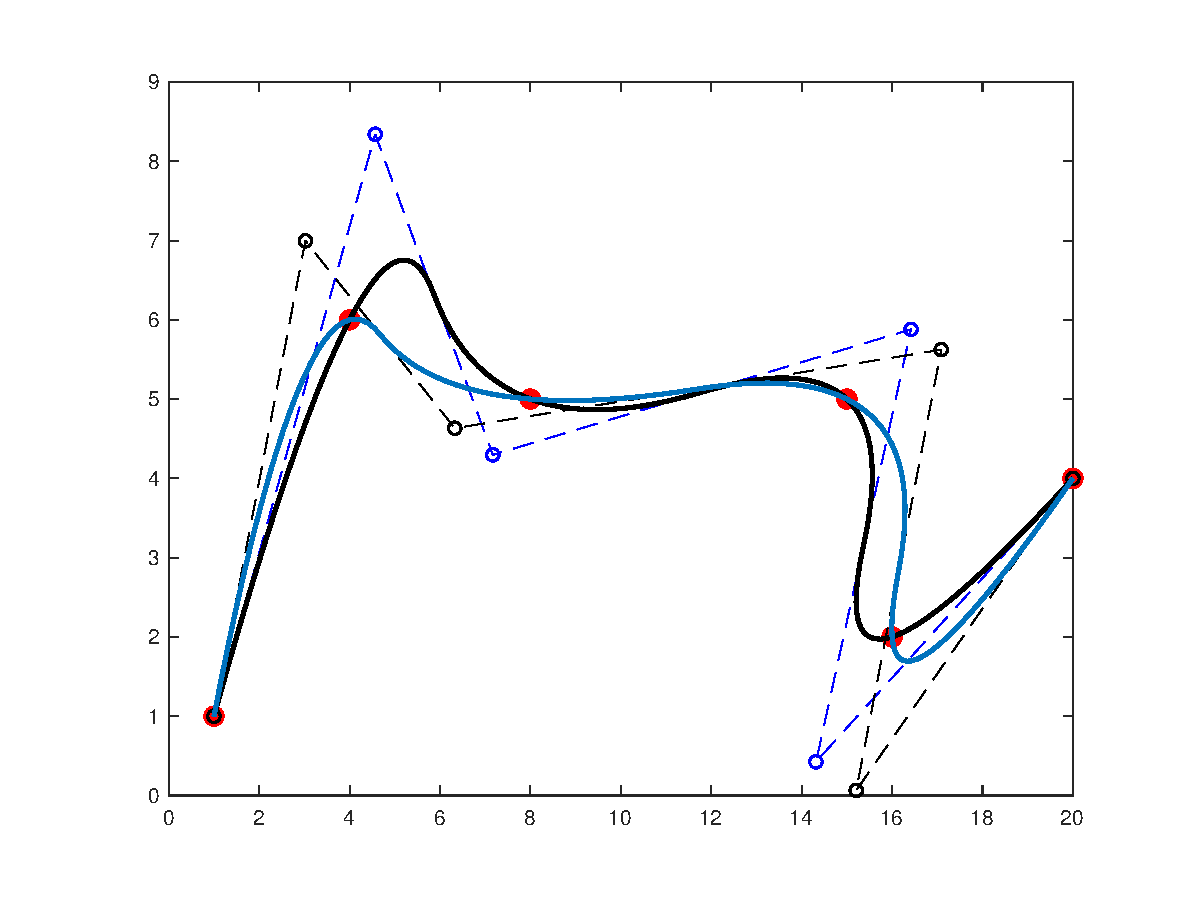
\includegraphics[width=0.75\textwidth]{figure/interpolation.eps}
  \caption{Interpolazione di punti}
  \label{fig:interpolation}
\end{figure} 


\section{Superfici}
\subsection{Superfici parametriche}
Una superficie può essere rappresentata attraverso la forma parametrica:
$$\mathbf{X}(u, v) = \begin{pmatrix}
  x(u, v) \\
  y(u, v) \\
  z(u, v)
\end{pmatrix}$$
con $u, v \in [a, b] \subset \mathbb{R}^2$.
La seguente superfice parametrica 
$$\mathbf{X}(u, v) = \begin{pmatrix}
  x(u, v) = (2 + cos(v)) \cdot cos(u)\\
  y(u, v) = (2 + cos(v)) \cdot sin(u)\\
  z(u, v) = sin(v)
\end{pmatrix}$$
è stata implementata in Codice~\ref{code:parametric_surface}. Il plot è visualizzato in Figura~\ref{fig:parametric_surface}.
\lstinputlisting[label=code:parametric_surface, firstline=2, lastline = 19, language=Matlab, caption = Disegno di una superficie parametrica]{code/parametric_surface.m}
\begin{figure}[]
  \centering
  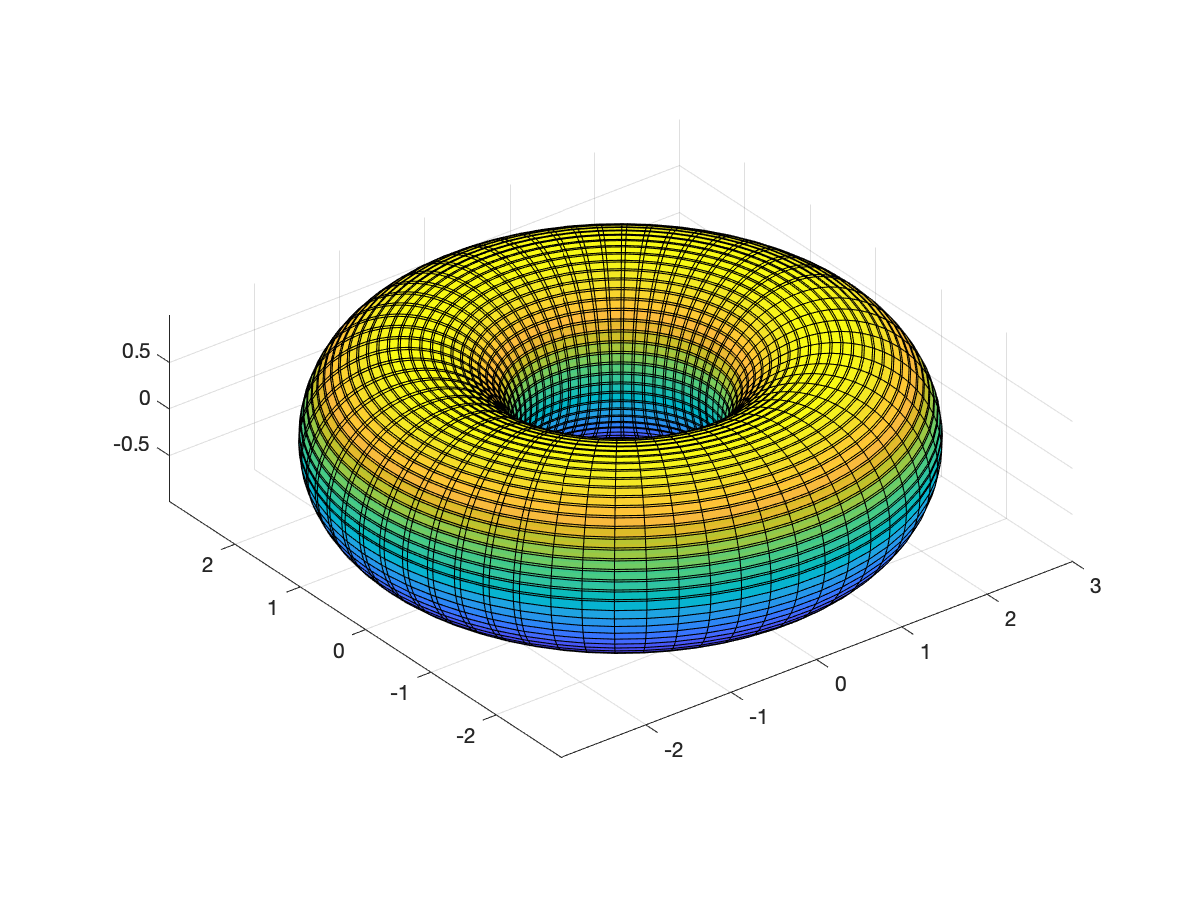
\includegraphics[width=0.75\textwidth]{figure/parametric_surface.eps}
  \caption{Supercifie parametrica}
  \label{fig:parametric_surface}
\end{figure} 
\subsection{Superfici \textit{Tensor-Product} di Bézier}
\begin{mydef}
  Dati due spazi di funzioni monovariate:
  $$S_1 = < B^{A}_{0}(u), \dots, B^{A}_{n}(u) > \qquad S_2 = < B^{B}_{0}(v), \dots, B^{B}_{m}(v) >$$
  con $u \in [a_A, b_A]$ e $v \in [a_B, b_B]$ si definisce uno spazio \textit{Tensor-Product} di funzioni bivariate come:
  $$S_1 \times S_2 = \left\{ f : \mathbb{R} \rightarrow \mathbb{R}: f(u, v) = \sum_{i = 0}^{n}\sum_{j = 0}^{m} c_{i,j}B^A_i(u)B^B_j(v) \right\}$$
  con $c_{i,j} \in \mathbb{R}$.
\end{mydef}
Una superficie \textit{Tensor-Product} di Bézier si definisce a partire dalla base di Bézier e da $(n+1)\cdot(m+1)$ vertici di controllo, i 
quali a loro volta formano un poligono di controllo. 
\begin{mydef}
  \label{def:tensor-prod-bez}
  Una superficie \textit{Tensor-Product} di Bézier è data da:
  $$\mathbf{X}(u, v) = \sum_{i = 0}^{n} \sum_{j = 0}^{m} \mathbf{b}_{i, j} B^{n}_{i}(u)B_{j}^{m}(v) $$
  dove:
  \begin{itemize}
    \item $B^{n}_{i}$ e $B^{m}_{j}$ sono i polinomi di Bernstein rispettivamente di 
    grado $n$ e $m$ e indice $i$ e $j$.
    \item $\mathbf{b}_{i,j}$ sono gli  $(n+1)\cdot(m+1)$ vertici di controllo.
  \end{itemize}
\end{mydef}
Di seguito, in Codice~\ref{code:bezier_basis} un'implementazione della base
per le superfici di Bézier realizzata con l'uso della funzione \texttt{spcol}.
\lstinputlisting[label=code:bezier_basis, firstline=2, language=Matlab, caption = Base delle superfici di Bézier]{code/bezier_surface_basis.m}
\lstinputlisting[label=code:bezier_surface, firstline=2, lastline = 19, language=Matlab, caption = Disegno di una superficie di Bézier]{code/bezier_surface.m}
\begin{figure}[]
  \centering
  \begin{subfigure}[b]{0.3\textwidth}
    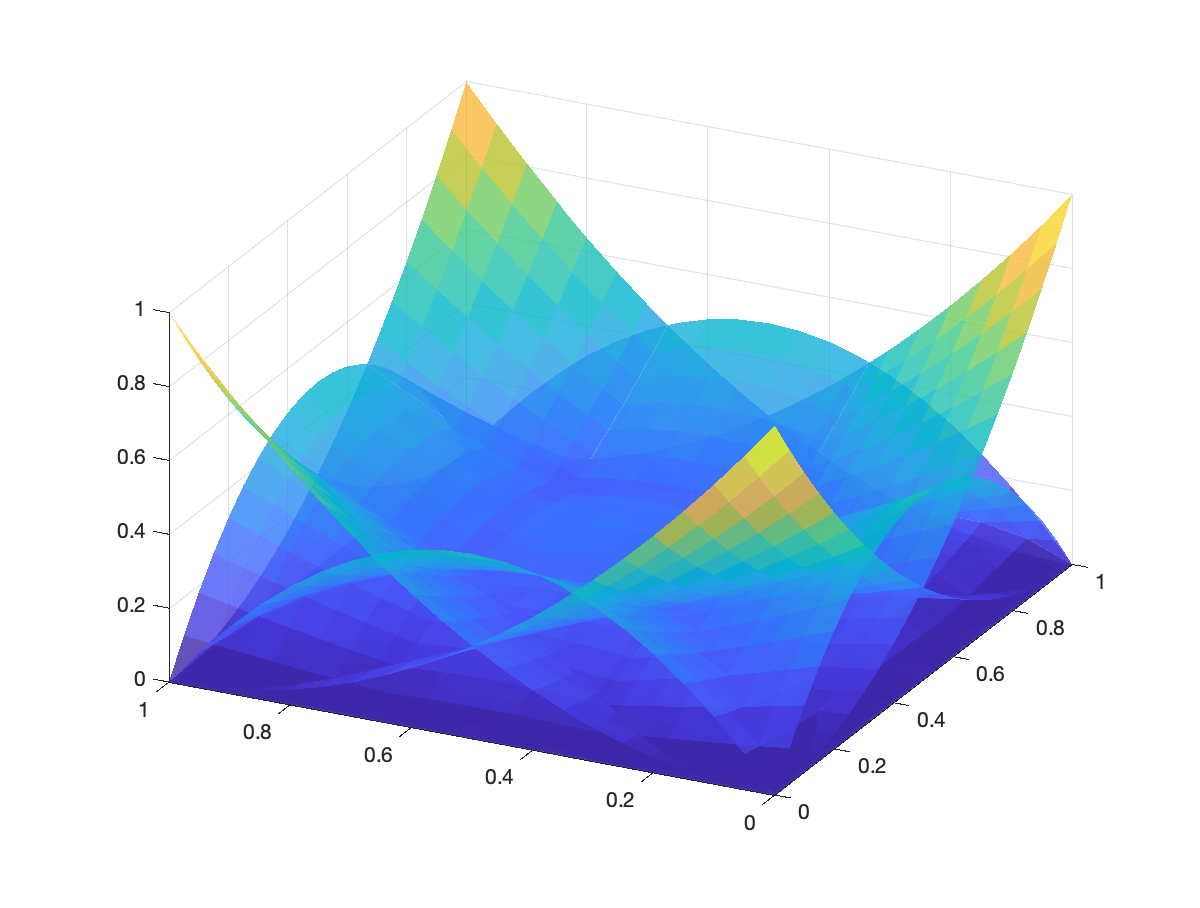
\includegraphics[width=\textwidth]{figure/bezier_surface_basis33_1.eps}
    \caption{$k_u$: $3$, $k_v$: $3$}
    \label{fig:bezier_surface_basis33_1}
  \end{subfigure}
  \begin{subfigure}[b]{0.3\textwidth}
      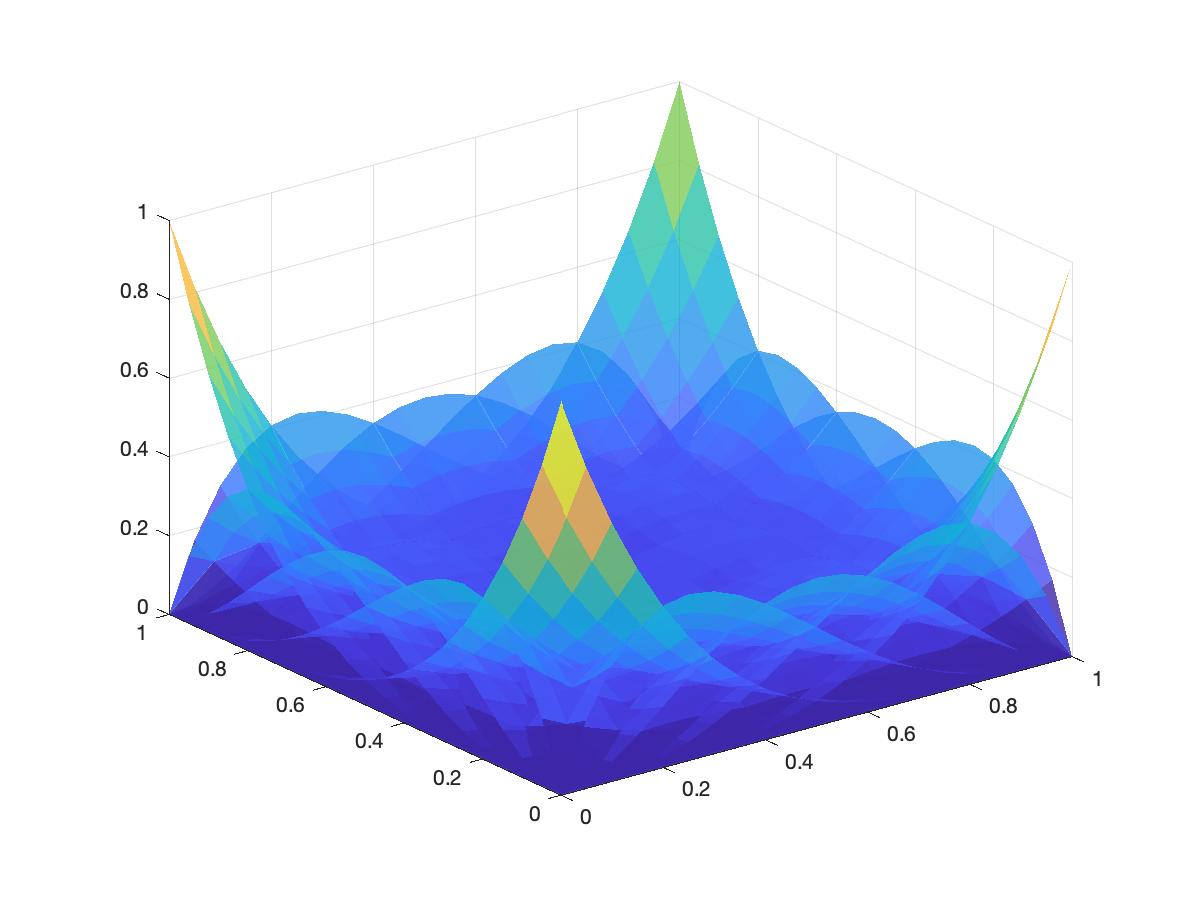
\includegraphics[width=\textwidth]{figure/bezier_surface_basis55_1.eps}
      \caption{$k_u$: $5$, $k_v$: $5$}
      \label{fig:bezier_surface_basis55_1}
  \end{subfigure}
  \begin{subfigure}[b]{0.3\textwidth}
      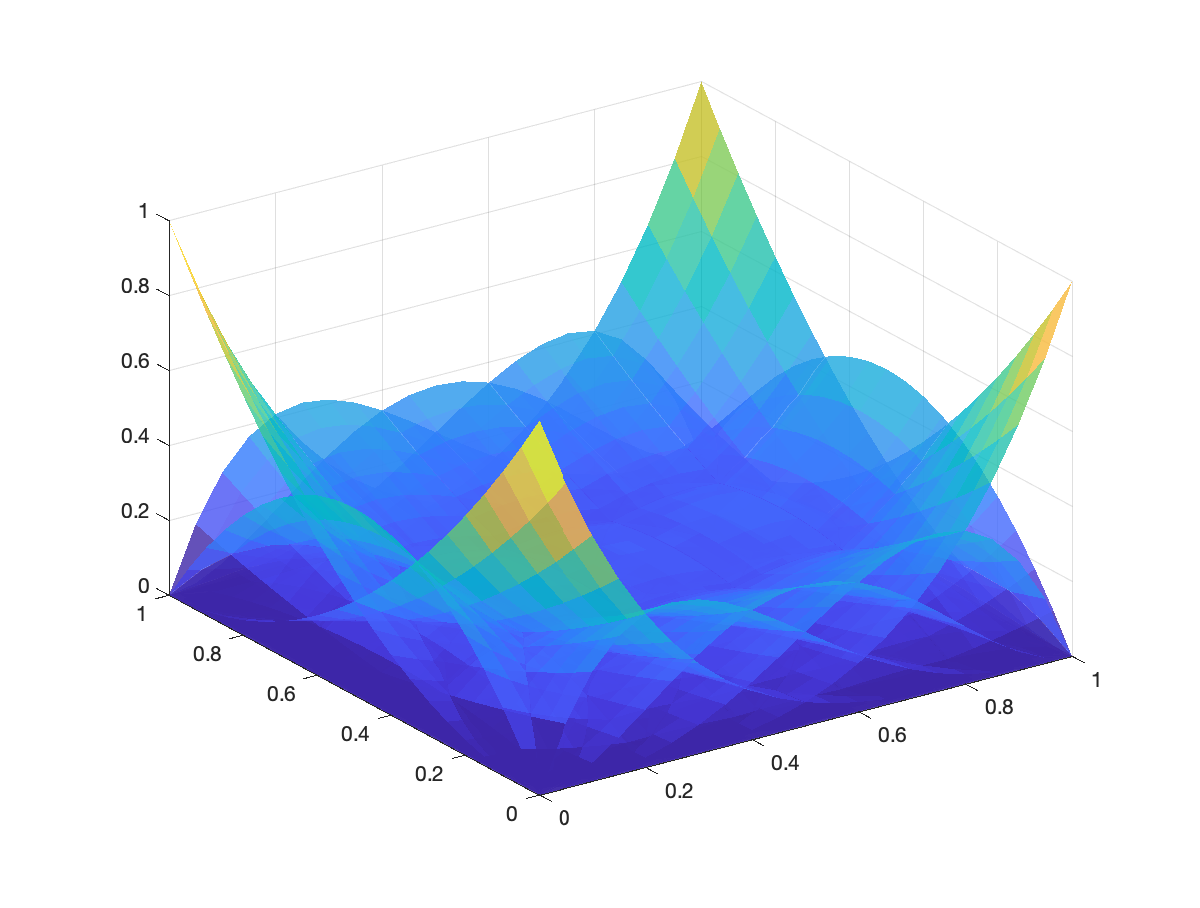
\includegraphics[width=\textwidth]{figure/bezier_surface_basis35_1.eps}
      \caption{$k_u$: $3$, $k_v$: $5$}
      \label{fig:bezier_surface_basis35_1}
  \end{subfigure}
  \caption{Base di Bézier}\label{fig:bezier_basis}
\end{figure}
\begin{figure}[]
  \centering
  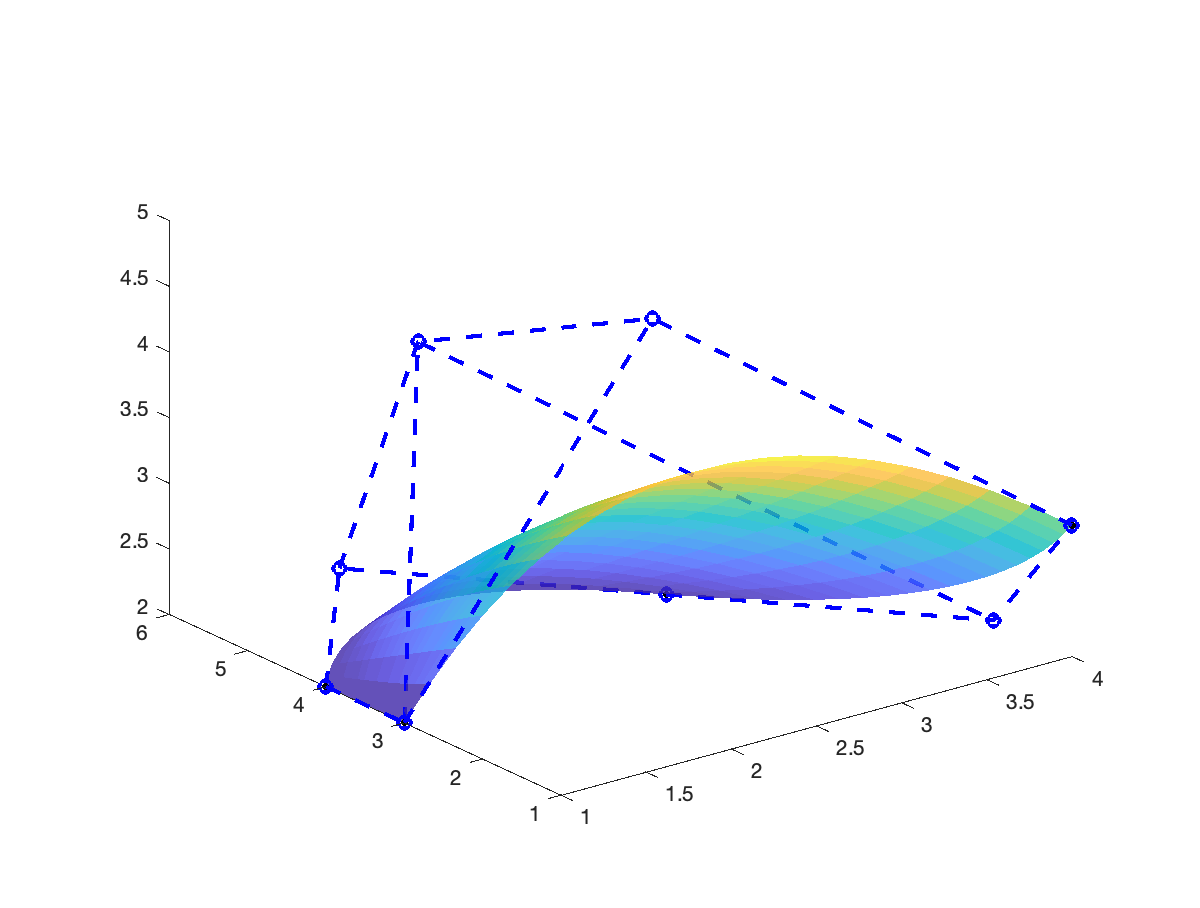
\includegraphics[width=0.75\textwidth]{figure/bezier_surface1.eps}
  \caption{Superficie di Bézier generata da Codice~\ref{code:bezier_surface}}
  \label{fig:bezier_sup_code}
\end{figure} 
\subsubsection{Proprietà delle superfici di Bézier}
Come per le curve, le superfici di Bèzier godono di alcune proprietà:
\begin{itemize}
  \item Invarianza per trasformazioni affini: applicare una trasformazione affine sui punti di controllo o sulla superfice è indifferente, il risultato sarà uguale.
  \item Curve di bordo: le quattro curve di bordo della superficie di Bézier sono date da
  $$\mathbf{X}(0,v) = \sum_{j=0}^{m} \mathbf{b}_{0,j}B_{j}^{m}(v) \quad \mathbf{X}(1,v) = \sum_{j=0}^{m} \mathbf{b}_{m,j}B_{j}^{m}(v)$$
  $$\mathbf{X}(u, 0) = \sum_{i=0}^{n} \mathbf{b}_{i,0}B_{i}^{n}(u) \quad \mathbf{X}(u,1) = \sum_{i=0}^{n} \mathbf{b}_{i, m}B_{i}^{n}(u)$$
\end{itemize}
  \paragraph{Invarianza per trasformazioni affini}
  Come detto in precedenza questa proprietà dice che applicare una trasformazione affine sui punti di controllo o sulla superfice è indifferente. 
  Questa proprietà risulta molto utile nella situazione in cui si deve applicare una determinata trasformazione ad una superficie. Il modo 
  più efficiente per realizzare ciò è applicare la trasformazione ai punti di controllo e successivamente ridisegnare la superfice.
  In Codice~\ref{code:bezier_surf_trans} è possibile vedere l'esempio di un disegno di una superficie e successiva trasformazione,
  sia sui punti di controllo che sulla superficie stessa.
  \lstinputlisting[label=code:bezier_surf_trans, firstline=2, lastline = 46, language=Matlab, caption = Trasformazione affine]{code/bezier_surface.m}
  In questo caso per mostrare che le due superfici trasformate sono uguali è stata usata la funzione \texttt{isequal}, che restituisce \texttt{1} se e solo se 
  le due matrici in input sono uguali. Il plot in output del Codice~\ref{code:bezier_surf_trans} è mostrato in Figura~\ref{fig:bezier_surf_trans}.
  \begin{figure}[]
    \centering
    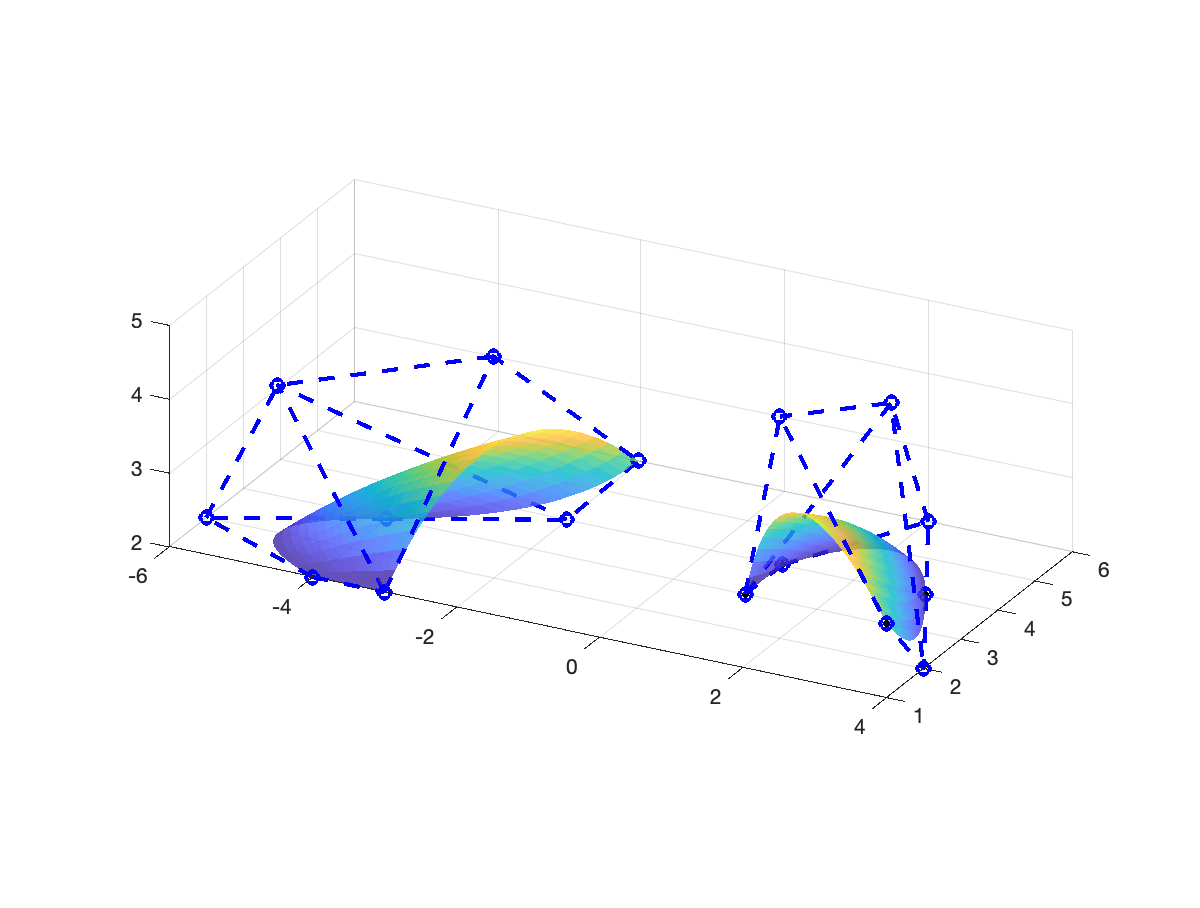
\includegraphics[width=0.75\textwidth]{figure/bezier_surf_trans.eps}
    \caption{Trasformazione affine su una superficie di Bézier}
    \label{fig:bezier_surf_trans}
  \end{figure} 
  \paragraph{Curve di bordo} I bordi di una superfice di Bézier possono essere visti a loro
  volta come quattro curve di Bézier:
  $$\mathbf{X}(0,v) = \sum_{j=0}^{m} \mathbf{b}_{0,j}B_{j}^{m}(v) \quad \mathbf{X}(1,v) = \sum_{j=0}^{m} \mathbf{b}_{m,j}B_{j}^{m}(v)$$
  $$\mathbf{X}(u, 0) = \sum_{i=0}^{n} \mathbf{b}_{i,0}B_{i}^{n}(u) \quad \mathbf{X}(u,1) = \sum_{i=0}^{n} \mathbf{b}_{i, m}B_{i}^{n}(u)$$
  In Codice~\ref{code:bezier_border_curve} è possibile vedere il calcolo, tramite l'algoritmo di \textit{De Casteljau}, di una delle quattro curve di bordo, 
  mentre in Figura~\ref{fig:bezier_border_curve} è possibile vedere 
  il plot dei bordi di una superficie di Bézier.
\begin{figure}[]
  \centering
  \begin{subfigure}[b]{0.3\textwidth}
    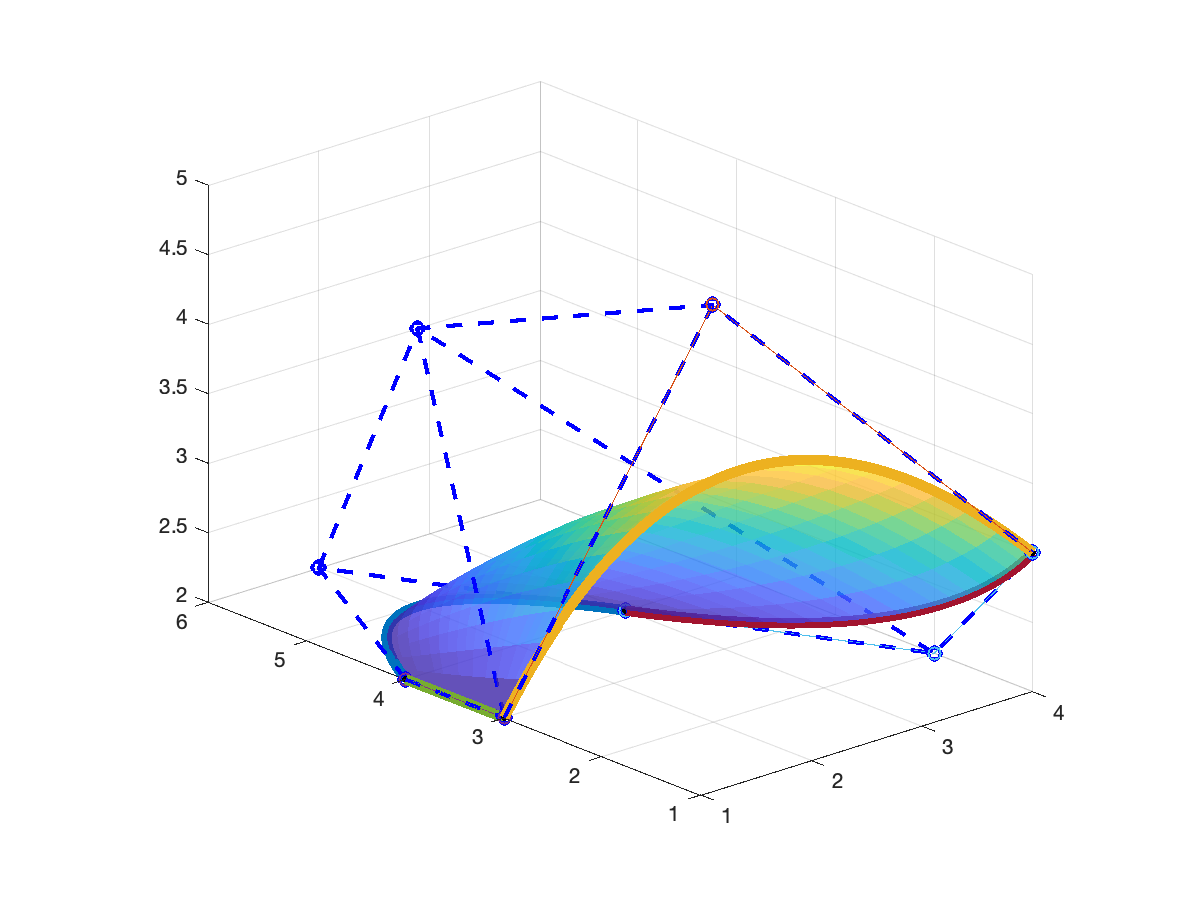
\includegraphics[width=\textwidth]{figure/border_curve.eps}
    \label{fig:border_curve}
  \end{subfigure}
  \begin{subfigure}[b]{0.3\textwidth}
      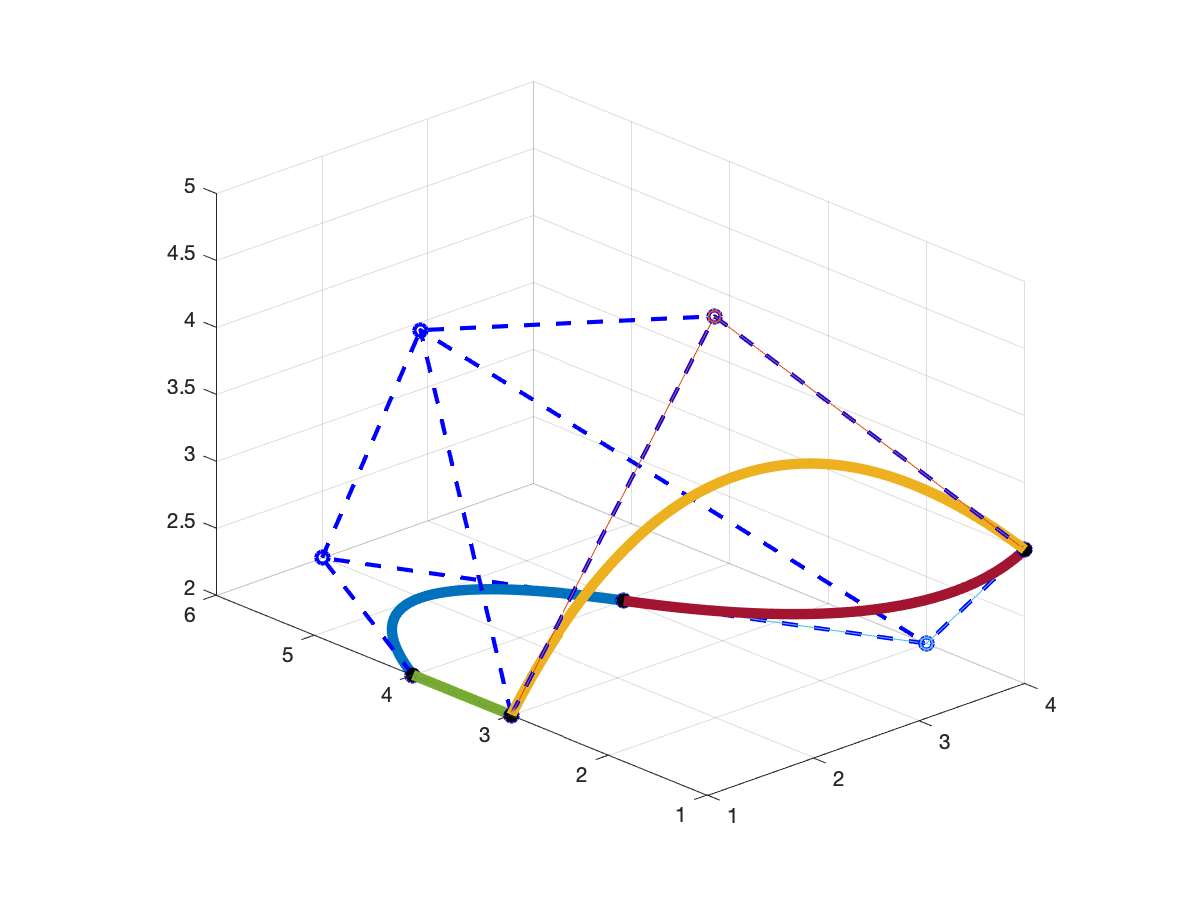
\includegraphics[width=\textwidth]{figure/border_curve_no_surf.eps}
      \label{fig:border_curve_no_surf}
  \end{subfigure}
  \begin{subfigure}[b]{0.3\textwidth}
      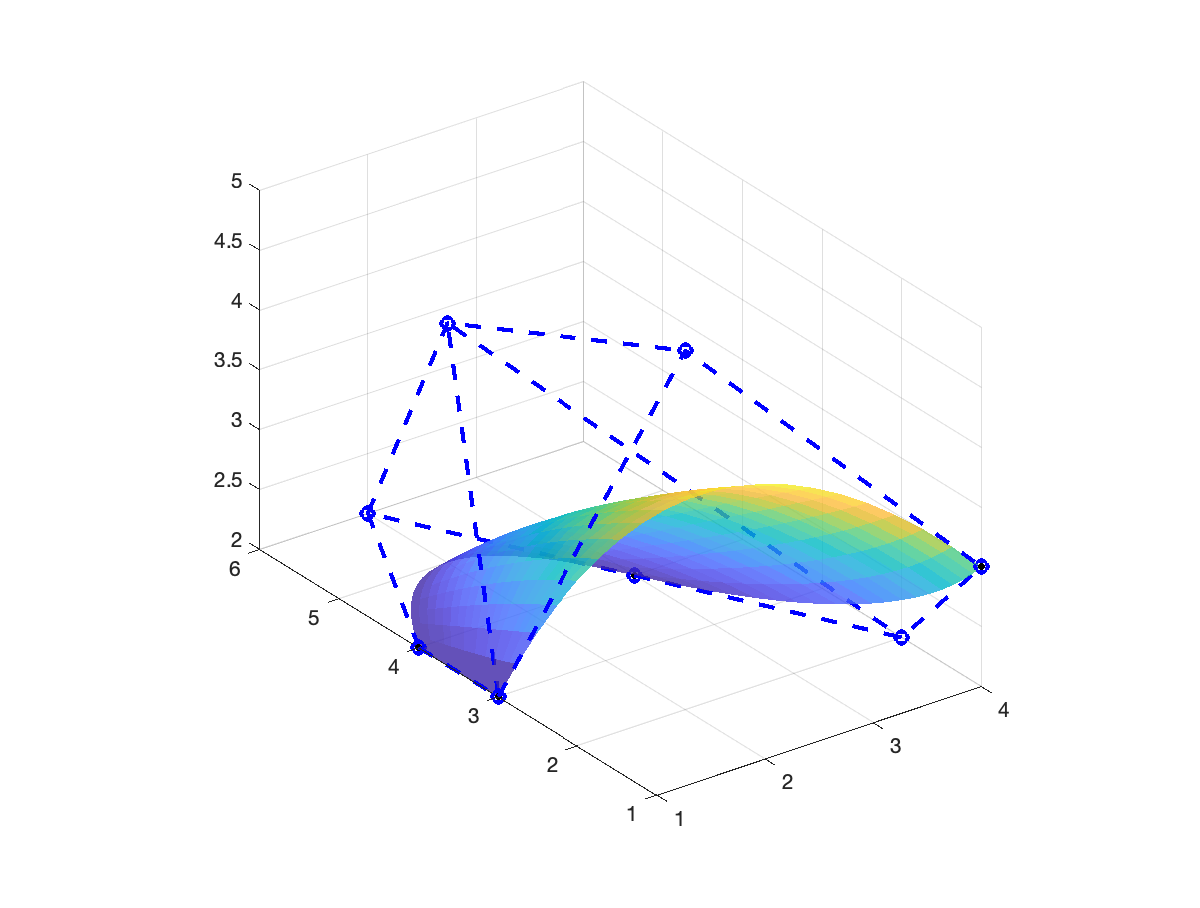
\includegraphics[width=\textwidth]{figure/surf_no_bord.eps}
      \label{fig:surf_no_bord}
  \end{subfigure}
  \caption{Curve di bordo}\label{fig:bezier_border_curve}
\end{figure}
\lstinputlisting[label=code:bezier_border_curve, firstline=76, lastline = 84, language=Matlab, caption = Curve di bordo]{code/bezier_surface.m}
\subsubsection{Algoritmo di De Casteljau}
Una superficie di Bézier, come definita in Definizione~\ref{def:tensor-prod-bez}, è possibile 
ottenerla tramite l'algoritmo di \textit{De Casteljau} eseguendo la seguente interpolazione bilineare.
$$\mathbf{b}^0_{i,j} = b_{i, j} \quad i = 0, \dots, n \quad j = 0, \dots, m$$
$$\mathbf{b}^{r,s}_{i,j}(u, v) = \begin{pmatrix} (1-u) & u\end{pmatrix}  \begin{pmatrix} \mathbf{b}^{r-1,s-1}_{i,j} & \mathbf{b}^{r-1,s-1}_{i,j+1} \\ \mathbf{b}^{r-1,s-1}_{i+1,j} & \mathbf{b}^{r-1,s-1}_{i+1,j+1}\end{pmatrix}  \begin{pmatrix}
  (1-v) \\ v
\end{pmatrix} $$
Eseguendo questa operazione sopra descritta si procede contemporaneamente in entrambe le direzioni $r$ ed $s$, 
quindi può essere eseguita un numero di volte massimo pari a
$\gamma = min(n, m)$, dopodiché è necessario procedere in una sola direzione eseguendo le iterazioni rimanenti.
L'approccio scelto per implementare l'algoritmo di 
\textit{De Casteljau} è descritto in \href{https://www.springer.com/la/book/9783642973857}{The NURBS Book}. 
L'algoritmo, implementato in Codice~\ref{code:disperazione}, \textit{non} procede in entrambe
le direzioni contemporaneamente, bensì prima in una e poi nell'altra. Acciocché questo possa essere reso possibile, 
è necessario dapprima implementare l'algoritmo per il disegno di curve per poi, successivamente, 
sfruttarlo per disegnare la superficie.
\lstinputlisting[label=code:disperazione, firstline=2, language=Matlab, caption = Algoritmo di De Casteljau]{code/disperazione.m}
Per accetarsi del corretto funzionamento dell'algoritmo implementato in Codice~\ref{code:disperazione}
sono state provate tutte le possibili casistiche riguardanti i gradi, ovvero:
\begin{itemize}
  \item $m > n$
  \item $n > m$
  \item $m = n$
\end{itemize}
In Figura~\ref{fig:surface_casteljau} è possibile vedere le tre diverse casistiche per i gradi delle superfici. I \textit{pallini} in rosso
sono i punti calcolati con l'algoritmo di \textit{De Casteljau}, e come \textbf{spero} sia possibile evidenziare si sovrappongono 
alla superfice disegnata in maniera convenzionale.
\begin{figure}[]
  \centering
  \begin{subfigure}[b]{0.6\textwidth}
    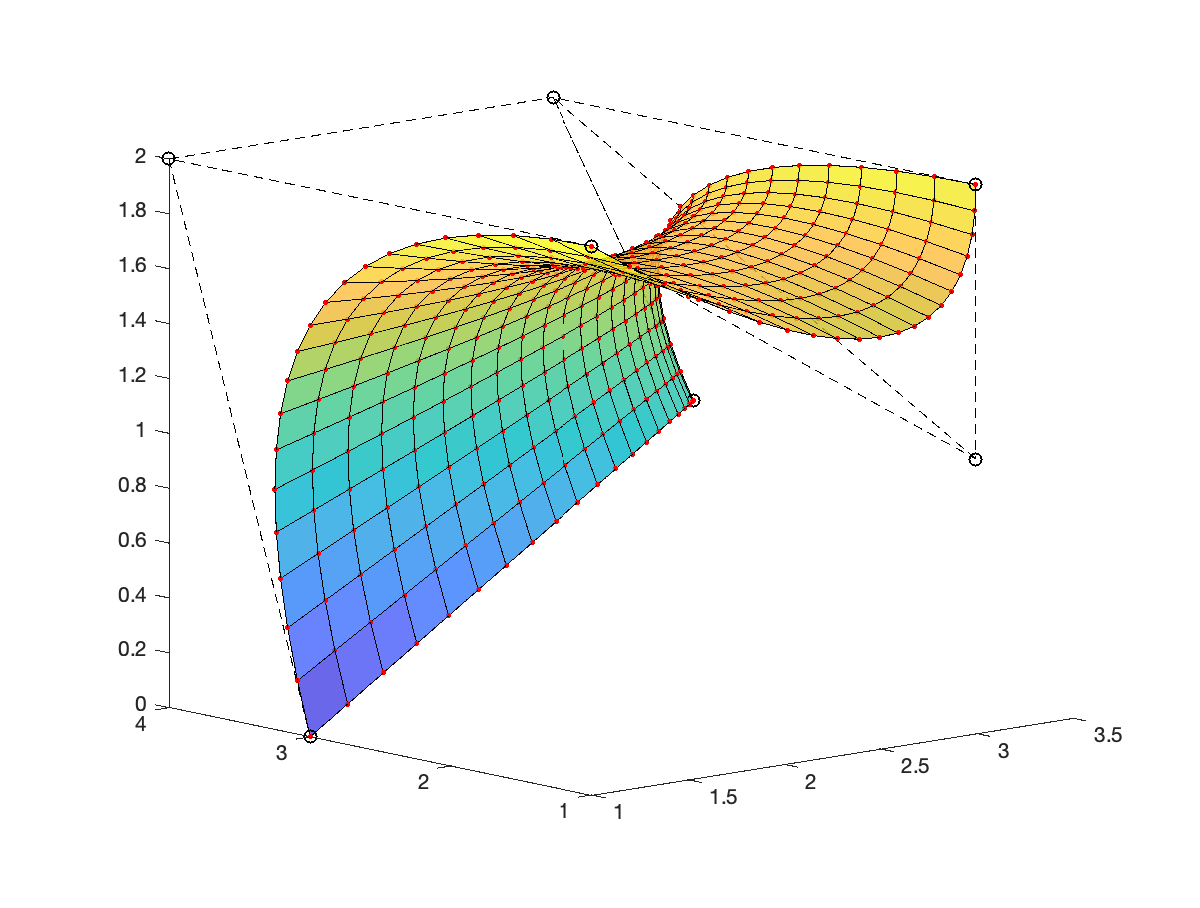
\includegraphics[width=\textwidth]{figure/surface_casteljau_m3n3.eps}
    \label{fig:surface_casteljau_m3n3}
    \caption{$m = 3, n = 3$}
  \end{subfigure}
  \begin{subfigure}[b]{0.6\textwidth}
      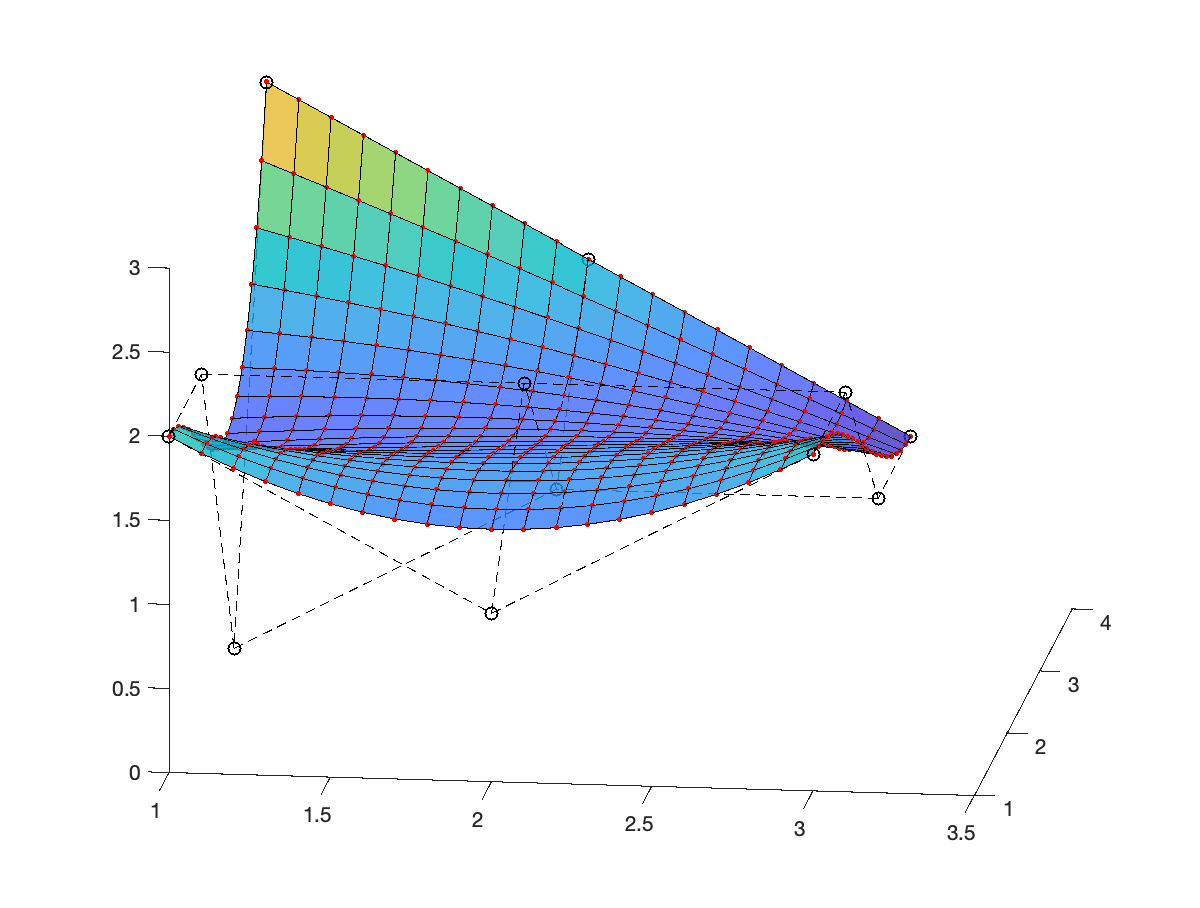
\includegraphics[width=\textwidth]{figure/surface_casteljau_m3n4.eps}
      \label{fig:surface_casteljau_m3n4}
      \caption{$m = 3, n = 4$}
  \end{subfigure}
  \begin{subfigure}[b]{0.6\textwidth}
      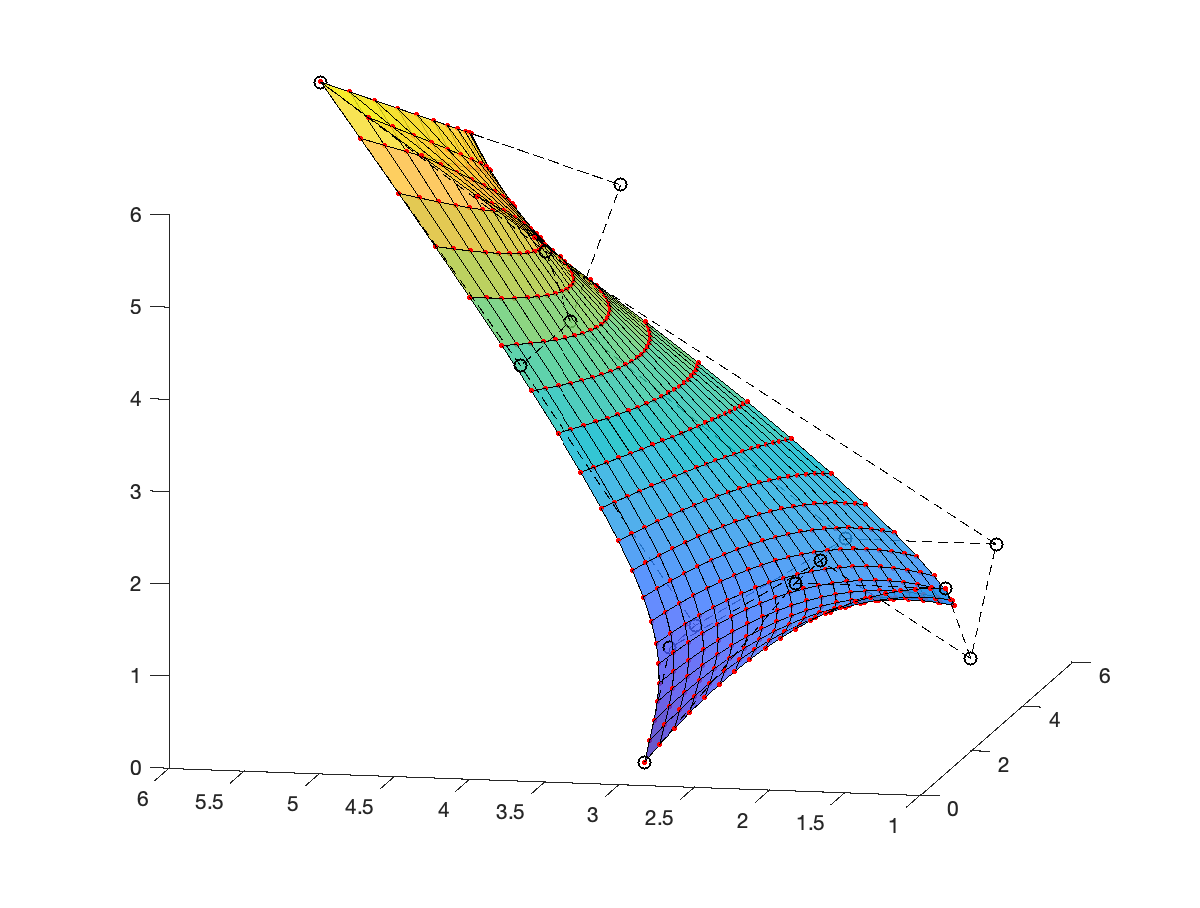
\includegraphics[width=\textwidth]{figure/surface_casteljau_m5n3.eps}
      \label{fig:surface_casteljau_m5n3}
      \caption{$m = 5, n = 3$}
  \end{subfigure}
  \caption{Superfici disegnate con \textit{De Casteljau}}\label{fig:surface_casteljau}
\end{figure}
\end{document}
